% !TeX root = ../report.tex

% Key information to be included:
% - Few lines about the general method and the steps followed
% - Heuristics (report the definitions in the previous slides)
% - Metrics agreed among all evaluators
% - Final scores agreed among all evaluators (include the main comments
% for your scores and examples of commentedscreenshots to support
% your scores)
% - Annex: Report the scores and main comments of EACH evaluator
% - PROVIDE AGGREGATED DATA, e.g., MEAN VALUES FOR ALL EURISTICS,
% (MEAN) SCORE BY DIMENSIONS (e.g., for CONTENT HEURISTICS,
% NAVIGATION HEURISTICS, ect.)
% - PROVIDE VISUAL REPRESENTATIONS OF RESULTS (diagrams, summary
% tables...)
% - Include a short conclusion section where you breifly discuss inspection
% results

\section{Inspection}

\subsection{Method}
% what is inspection based usability evaluation
% specific heuristics and metrics used
Inspection-based usability evaluation allows teams of evaluators to perform
a systemic analisys of UI/UX aspects of an application (a website, in our case).
We adopted the widely used \emph{heuristic evaluation}, as the main usability inspection method, in which the evaluators concentrate on a set of principles (``heuristics'') to test the usability of the application.

\subsubsection{Heuristics}

This section explains the different heuristics we adopted to evaluate the
website compliance to usability quality principles. In particular, we used
\emph{Nielsen's} and a subset of \emph{MiLE} (Milano Lugano usability Evaluation method) heuristics.

\paragraph*{Nielsen's heuristics}

\begin{enumerate}[start=1,label={\bf H\arabic{*}}]
    \item \textbf{Visibility of system status:} does the user know where they are and    
          what's going on?
    \item \textbf{Match between system and the real world:} does the system use 
          conventions known to the users?
    \item \textbf{User control and freedom:} can the user leave unwanted state quickly? 
          Is undo/redo available to them?
    \item \textbf{Consistency and standards:} do multiple words/elements/actions mean    
          the same thing?
    \item \textbf{Error prevention:} do the application try to prevent problems 
          from occurring (e.g.: checking inputs before submitting them)?
    \item \textbf{Recognition rather than recall:} are options visible or easily 
          retrievable?
    \item \textbf{Flexibility and efficiency of use:} are accelerators available?
    \item \textbf{Aesthetic and minimalist design:} is dialogue containing only relevant 
          informations?
    \item \textbf{Help users recognize, diagnose and recover from errors:} are error 
          codes in plain language? Do they suggest a possible solution?
    \item \textbf{Help and documentation:} (if any) is it easily searchable?
\end{enumerate}

\paragraph*{MiLE heuristics}

We can further subdivide MiLE heuristics in 3 categories: navigation, content, presentation.

\subparagraph*{Navigation}

\begin{enumerate}[start=1,label={\bf MN\arabic{*}}]
    \item \textbf{Interaction consistency:} do pages of the same type have the same links
          and interaction capability?
    \item \textbf{Group navigation:} is it easy to navigate from and among groups of
          ``items''?
    \item \textbf{Structural Navigation:} is it easy to navigate among the ``components'' of a topic?
    \item \textbf{Semantic Navigation:} is it easy to navigate between related topics?
    \item \textbf{Landmarks:} are landmarks useful to reach the key parts of the web
          site?
\end{enumerate}

\subparagraph*{Content}

\begin{enumerate}[start=1,label={\bf MC\arabic{*}}]
    \item \textbf{Information overload:} is the information in a page too much/too
          little?
\end{enumerate}

\subparagraph*{Presentation}

\begin{enumerate}[start=1,label={\bf MP\arabic{*}}]
    \item \textbf{Text lay out:} is the text readable? Is font size appropriate?
    \item \textbf{Interaction placeholders-semiotics:} are textual or visual    
          labels of interactive elements ``expressive'' and meaningful?
    \item \textbf{Interaction placeholders-consistency:} are textual or visual 
          labels of interactive elements consistent in terms of wording, icon, 
          position, etc.?
    \item \textbf{Spatial allocation:} is the on-screen allocation of contents 
          and visual appropriate for their relevance? Are ``semantically 
          related'' elements close and ``semantically distant'' element far 
          away?
    \item \textbf{Consistency of Page Structure:} do pages of the same type 
          have the same layout?
\end{enumerate}

\subsubsection{Metrics}

To keep the inspection process straightforward, we agreed on evaluating the compliance of the website to each heuristic on a scale from 0 to 3, without decimals. In this way, we avoid situations where it's hard to define the difference two close numbers on larger scales (e.g.: 6 and 7 on a scale from 1 to 10).

\begin{figure*}[h]
    \begin{tabular}{c l l}
        \toprule
        \textbf{Score} & \textbf{Meaning} & \textbf{Comment} \\
        \midrule
        0 & Bad & Heuristic not satified at all \\
        1 & Worse than better & There are multiple violations of the heuristic \\
        2 & Better than worse & Overall the heuristic is satified with some  exception \\
        3 & Good & Heuristic satified\\
        \bottomrule
    \end{tabular}
\end{figure*}

Since not all heuristics apply in all situations, we could also assign a ``N/A'' (``not applicable'') in such cases.

\subsection{Execution of the study}
In order to identify a relevant subset of URLs of the website to analyze during the inspection, we agreed on proceeding in the following way:
\begin{itemize}
    \item we selected together the main functionalities of the website and identified relevant tasks related to them
    \item for each task, we identified three to four URLs that might be involved in accomplishing the task    
\end{itemize}
Having defined a basic subset of URLs as stated above, we individually performed the inspection for each heuristic. We assigned a score and provided a short comment. \\
It has to be noted that the subset of URLs was used as a common ground, but each inspector widened the spectrum of analysis as he considered appropriate.\\
Finally, we discussed the results together and made a synthesis of our evaluation, agreeing on a final score for each heuristic.   


\pagebreak

\subsection{Results}
Inspection was initially carried out individually by each evaluator. At the end of this first phase, a meeting was held in order to reach an agreed score for each heuristic.\\
We report thre results in a summary table grouping each heuristics into rows with their corresponding agreed score and comment, more detailed comments for each heuristic with examples will be illustrated in the next section.\\
It must be noticed that the final scores agreed on usually differed from the arithmetic mean: the level of disagreement over each topic (represented by the variance) was also considered. A graphical visualization is also provided, highlighting both the mean and the variance (Fig. \ref{BarsNielsenCrop} and Fig. \ref{BarsMileCrop}).

\begin{tabularx}{\linewidth}{l c X}
\toprule
\textbf{Heuristic} & \textbf{Score} & \textbf{Comment} \\
\midrule
\endfirsthead
\toprule
\textbf{Heuristic} & \textbf{Score} & \textbf{Comment} \\
\midrule
\endhead
\midrule
\footnotesize [Continues on next page]
\endfoot
\bottomrule
\endlastfoot
    % body
    H1 & 1 & There is a difficulty in navigation as breadcrumbs are sometimes either missing or incorrect.\par When using the search bar, there is no feedback on the progress status, the page can appear frozen. \\ \midrule
    H2 & 2 & Some visual and textual elements are confusing and do not match the real world in a proper way.\\ \midrule
    H3 & 0 & If we consider only the main site, which mainly provides information, this heuristic is not applicable.\par Major problems can be found in the hotel subsection.\\ \midrule
    H4 & 2 & Some icons and buttons don't follow certain conventions and there are cases in which they provide different functionalities across different pages, hence they are not even consistent.\\ \midrule
    H5 & 2 & Error prevention is not always implemented, mainly in the newsletter subscription form and in the registration process suggestions are not always present.\\ \midrule
    H6 & 3 & No major problems detected in this heuristic.\\ \midrule
    H7 & 1 & Detected issues mainly related to landmarks, see MN5.\\ \midrule
    H8 & 2 & Presence of an huge banner at the top of the pages is not a good design choice as it takes space from relevant information at its bottom.\\ \midrule
    H9 & 2 & Helpful messages for error recognition are not always provided.\\ \midrule
    H10 & N/A & Heuristic not applicable to the site
\end{tabularx}

\begin{figure}[!ht]
    \begin{minipage}{\linewidth}
        \centering
        \makebox[\textwidth][c]{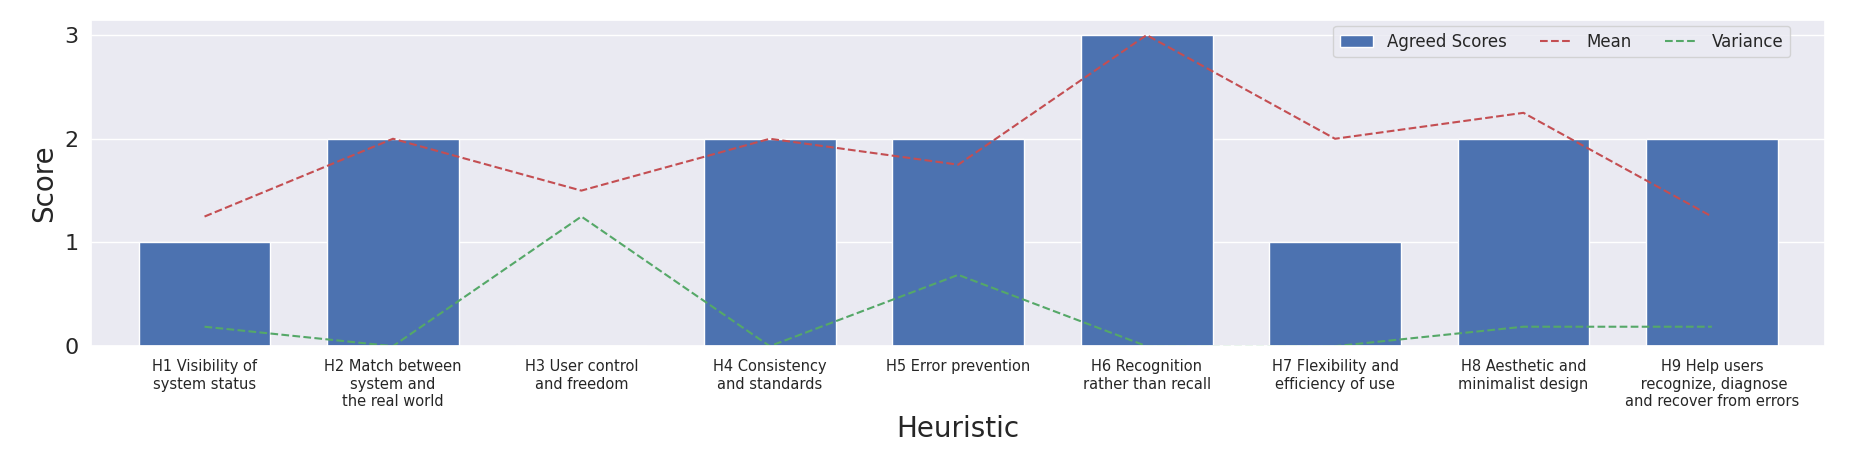
\includegraphics[width=1.2\textwidth]{images/BarsNielsenCrop.png}}%
        \captionsetup{justification=centering}
        \caption{Nielsen's heuristics evaluation summary}
        \label{BarsNielsenCrop}
    \end{minipage}
\end{figure}

%\paragraph{MiLe}

\pagebreak

\begin{tabularx}{\linewidth}{l c c X}
\toprule
\textbf{Category} & \textbf{Heuristic} & \textbf{Score} & \textbf{Comment} \\
\midrule
\endfirsthead
\toprule
\textbf{Category} & \textbf{Heuristic} & \textbf{Score} & \textbf{Comment} \\
\midrule
\endhead
\midrule
\footnotesize [Continues on next page]
\endfoot
\bottomrule
\endlastfoot

\multirow{5}{*}{\textbf{Navigation}}   & MN1 & 3 & Similar pages have the same type of layout, links and interaction capabilities\\ \cmidrule{2-4} 
                                        & MN2 & 3 & Navigation from a group to its items is quite easy, while the opposite is not always possible.\\ \cmidrule{2-4} 
                                        & MN3 & 2 & Many pages force the user to scroll back to the top of the page in order to use the page anchors for structural navigation.\\ \cmidrule{2-4} 
                                        & MN4 & 2 & Navigating from a topic to a related one is easy, but navigating backward is not possible unless through the browser's back arrow.\\ \cmidrule{2-4} 
                                        & MN5 & 1 & Major problems with the landmarks, mostly presence of useless ones and absence of more useful kinds.\\ \midrule
\textbf{Content}                       & MC1 & 1 & Critical information overload in certain pages \\ \midrule
\multirow{5}{*}{\textbf{Presentation}} & MP1 & 3 & The text is always readable and of the appropriate size. \\ \cmidrule{2-4} 
                                        & MP2 & 2 & Some labels and and icons are not expressive enough and do not reflect the meaning of the interaction and its effects.\\ \cmidrule{2-4} 
                                        & MP3 & 2 & Some interactive elements are inconsistent in terms of wording and icon.\\ \cmidrule{2-4} 
                                        & MP4 & 1 & Some critical and useful information and links are allocated in in a bad way.\\ \cmidrule{2-4} 
                                        & MP5 & 3 & No major problems, pages of the same type have the same layous.
\end{tabularx}

\begin{figure}[!ht]
    \begin{minipage}{\linewidth}
        \centering
        \makebox[\textwidth][c]{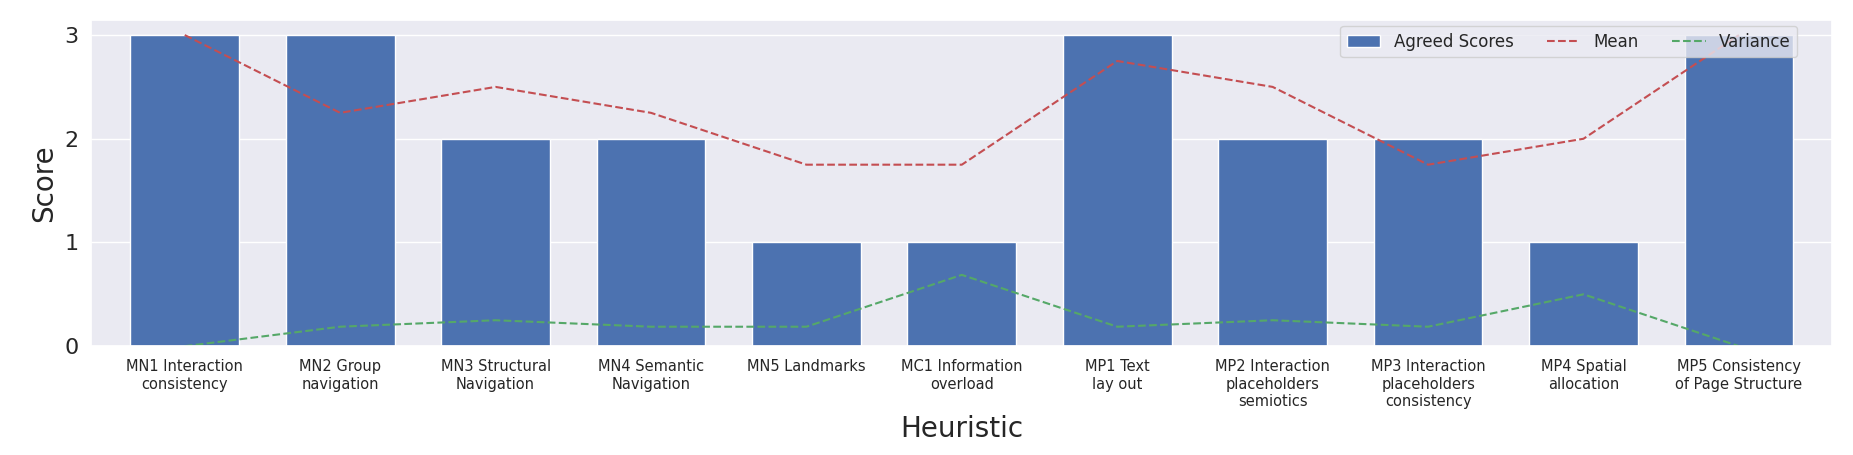
\includegraphics[width=1.2\textwidth]{images/BarsMileCrop.png}}%
        \captionsetup{justification=centering}
        \caption{MiLe's heuristics evaluation summary}
        \label{BarsMileCrop}
    \end{minipage}
\end{figure}

\pagebreak

Finally, mean values by content, navigation and presentation heuristics are provided in Fig. \ref{BarsAggregated}.\\
There is an overall consensus that the website presents major problems on the content part. Explanations will be tackled in the next sections. 

\begin{figure}[!ht]
    \begin{minipage}{\linewidth}
        \centering
        \makebox[\textwidth][c]{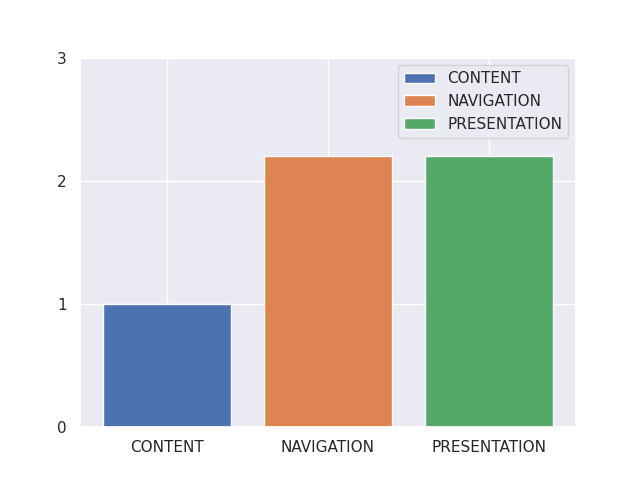
\includegraphics[width=0.6\textwidth]{images/BarsAggregated.png}}%
        \captionsetup{justification=centering}
        \caption{Aggregated heurstics data by dimensions}
        \label{BarsAggregated}
    \end{minipage}
\end{figure}

\subsection{Discussion of results}
\subsubsection{Discussion within Nielsen's heuristics}
\begin{itemize}
    \item \textbf{H1 Visibility of system status}\\
        The orientational information of the website is often incomplete or misleading. This is mainly due to the inconsistent use of bread crumbs, which are sometimes missing.\\
        We also found out that depending on the navigation history, bread crumbs might be incorrect as well, since they are not sufficiently dynamic. An example of this issue is the fact that we reached the page in Fig. \ref{H1-1} from the home page but the bread crumbs are erroneous.\\
        Another issue is related to the search bar provided as a landmark. The system does not provide feedback on the status of the research process. In fact, the page looks frozen and this might lead the user to reload the page (Fig. \ref{H1-2}).\\
        \begin{figure}[!ht]
            \begin{minipage}{\linewidth}
                \centering
                \makebox[\textwidth][c]{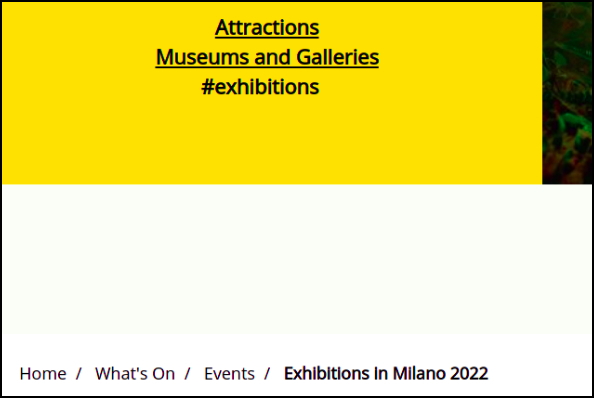
\includegraphics[width=0.5\textwidth]{images/H1-1.png}}%
                \captionsetup{justification=centering}
                \caption{An example of incorrect breadcrumbs.}
                \label{H1-1}
            \end{minipage}
        \end{figure}
        \begin{figure}[!ht]
            \begin{minipage}{\linewidth}
                \centering
                \makebox[\textwidth][c]{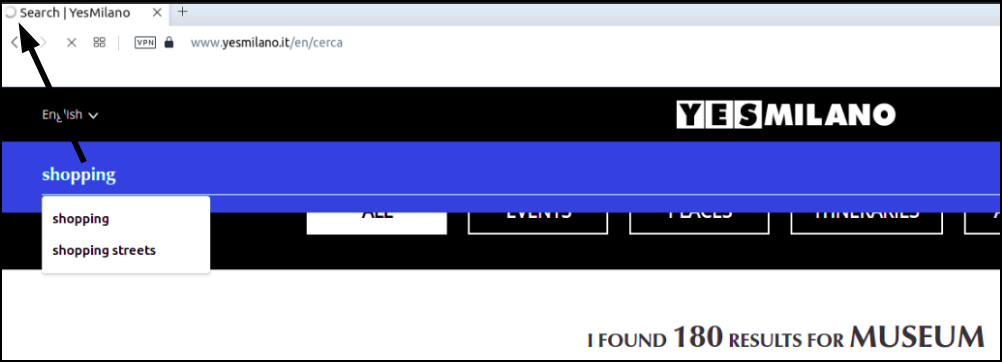
\includegraphics[width=1\textwidth]{images/H1-2.png}}%
                \captionsetup{justification=centering}
                \caption{The page is loading but it appears to be frozen.}
                \label{H1-2}
            \end{minipage}
        \end{figure}
    \pagebreak
    \item \textbf{H2 Match between system and the real world}
        Regarding the match between the system and the real world, the heuristic is generally satisfied. Visual representations for specific sections are quite effective (e.g. showing pictures of art exhibitions as thumbnails for the art section in the home page, the picture of a student for the study section). However, minor inconsistencies were detected, such as:
        \begin{itemize}
            \item the presence of topic-unrelated pictures in the Coronavirus Info page (see Fig. \ref{H2-1})
            \item in Castello Sforzesco's page some search words in the top section of the page are not related to the content of the page itself (e.g. top/my first trip to Milano is not related to Castello Sforzesco in the real world)
        \end{itemize}
        \begin{figure}[!ht]
            \begin{minipage}{\linewidth}
                \centering
                \makebox[\textwidth][c]{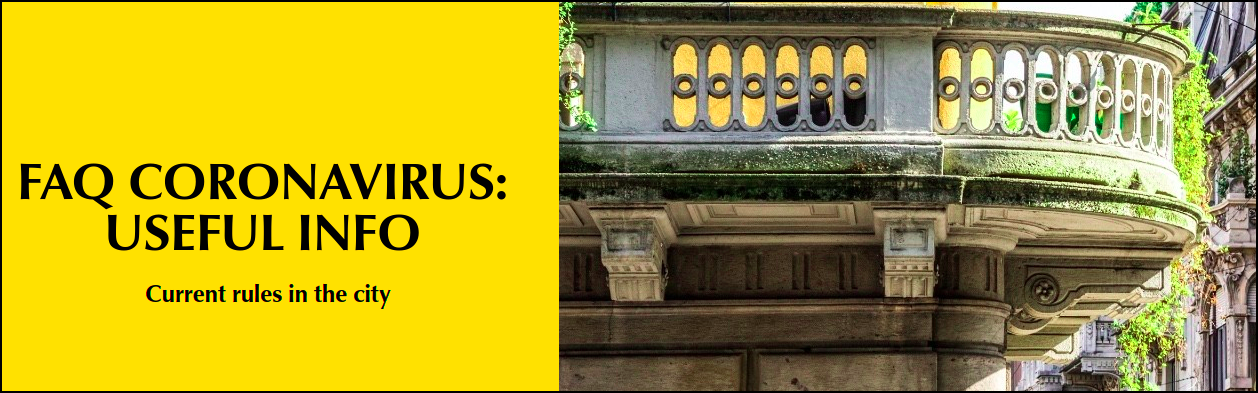
\includegraphics[width=1\textwidth]{images/H2-1.png}}%
                \captionsetup{justification=centering}
                \caption{The content of a page and the image used are unrelated.}
                \label{H2-1}
            \end{minipage}
        \end{figure}
    \item \textbf{H3 User control and freedom}\\
        For most of the pages of the website this heuristic can be considered as not applicable, since the main purpose of the website is to provide information. The support of undo and redo operations is almost never required.\\
        Still, one issue was detected in the hotel section: when the user inserts the information required in order to book a room (such as the number of guests, etc.) the user is redirected to another page, with no possibility to modify those parameters without having to reload the previous page (and by doing so, refill all the parameters).
    \item \textbf{H4 Consistency and standards}\\
        The website is generally consistent and follows standards with the proficient use of icons (see Fig. \ref{H4-1}). We identified some minor issues:
        \begin{itemize}
            \item sometimes a "+" button (Fig. \ref{H4-2}) is used but it has an unexpected behavior: it should extend the number of items shown whereas it redirects the user to another page
            \item "-" and "x" symbols are both use to compress contents
            \item in some pages (e.g. Coronavirus FAQ) some icons are clickable but don't perform anything (such as the contacts icon)
            \item in some specific restaurant pages two different icons for reservation are used
            \item in some pages the table of content/index is not following a standard style but is centered at the top of the page, as shown in Fig. \ref{H4-3}
        \end{itemize}
        \begin{figure}[!ht]
            \begin{minipage}{\linewidth}
                \centering
                \makebox[\textwidth][c]{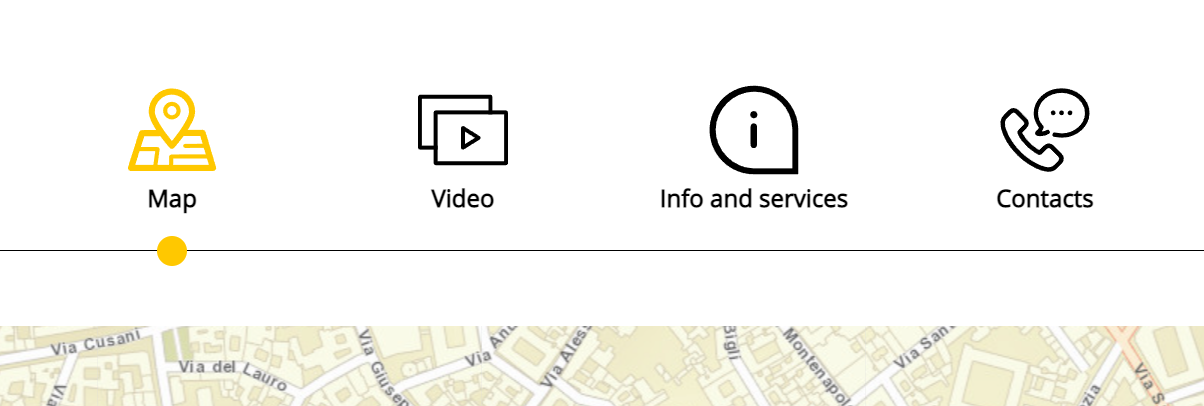
\includegraphics[width=1\textwidth]{images/H4-1.png}}%
                \captionsetup{justification=centering}
                \caption{An example of good use of conventions.}
                \label{H4-1}
            \end{minipage}
        \end{figure}
        \begin{figure}[!ht]
            \begin{minipage}{\linewidth}
                \centering
                \makebox[\textwidth][c]{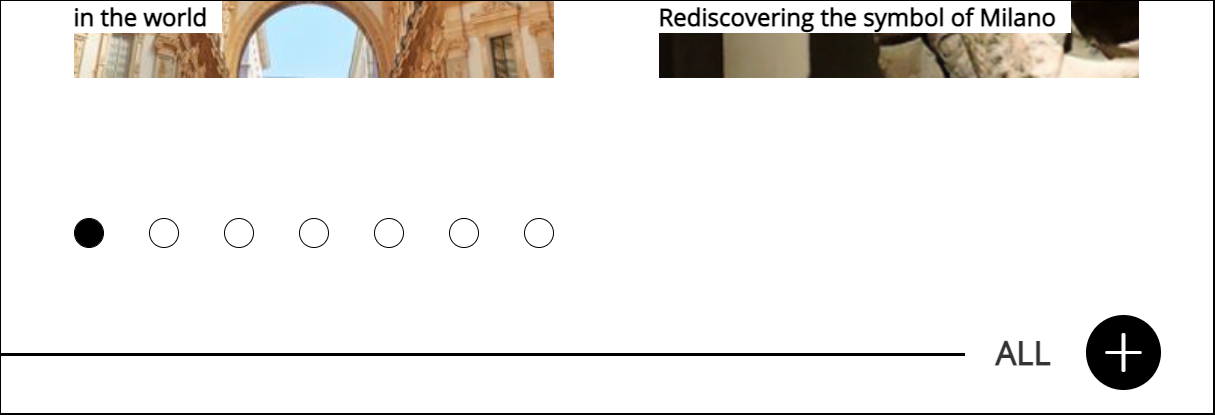
\includegraphics[width=1\textwidth]{images/H4-2.png}}%
                \captionsetup{justification=centering}
                \caption{A "+" icon with unexpected behavior.}
                \label{H4-2}
            \end{minipage}
        \end{figure}
        \begin{figure}[!ht]
            \begin{minipage}{\linewidth}
                \centering
                \makebox[\textwidth][c]{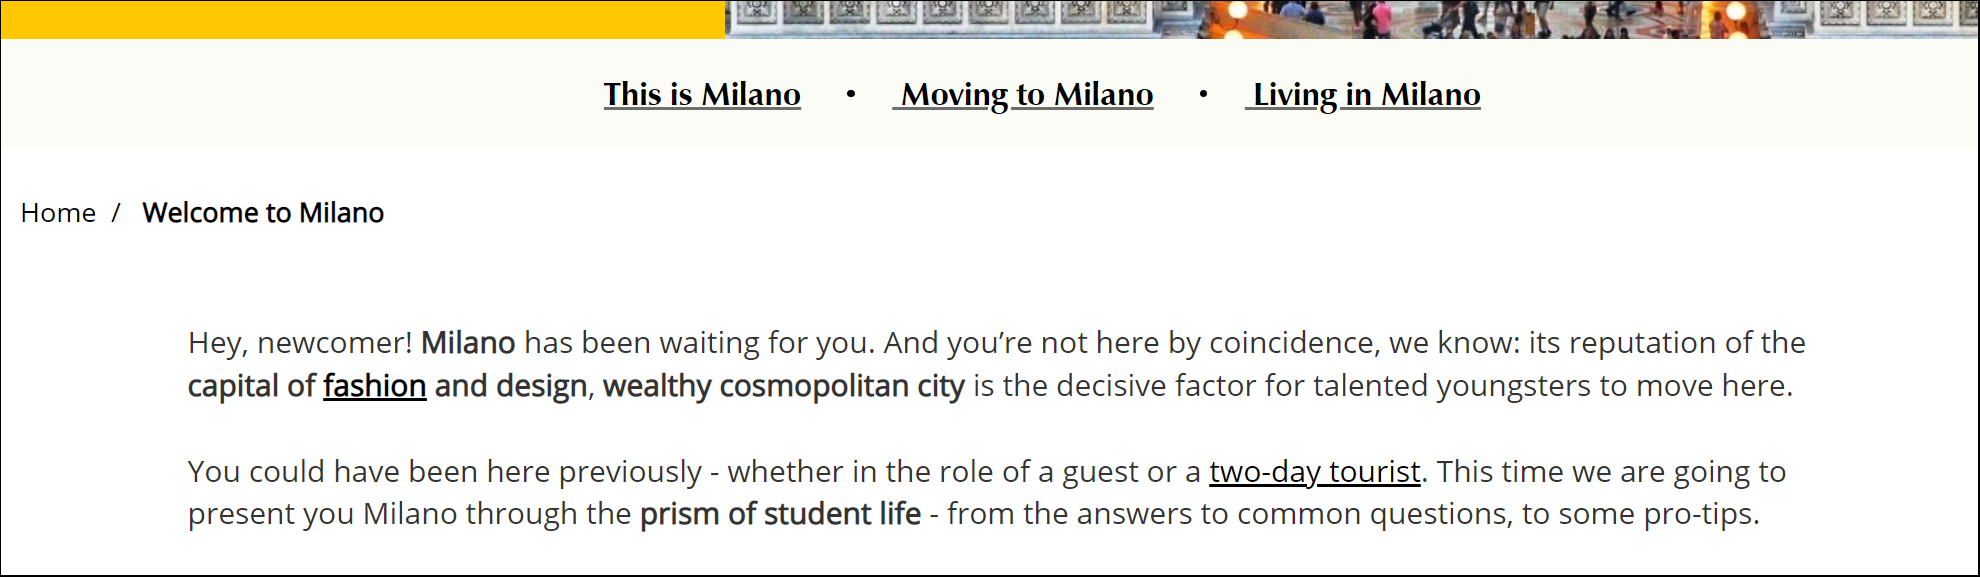
\includegraphics[width=1\textwidth]{images/H4-3.png}}%
                \captionsetup{justification=centering}
                \caption{Table of contents that does not follow a standar.}
                \label{H4-3}
            \end{minipage}
        \end{figure} 
    \item \textbf{H5 Error prevention}\\
        Regarding error prevention, two minor problems were detected.\\
        The first is the fact that in the newsletter form, the table reservation form and the research bar the user is not informed by a warning about the fact that some fields are blank. This might lead the user to proceed with the form with missing inputs.
        The second is that in the student registration no suggestion is provided in case of an email written with a missing "@".\\        
        For what concerns the overall website, getting to the wrong page is most of the time avoided by meaningful link labels.
    \item \textbf{H6 Recognition rather than recall}\\
        This heuristic is fully satisfied in fact all the search forms suggest options for recognition.
    \item \textbf{H7 Flexibility and efficiency of use}\\
        ???
    \item \textbf{H8 Aesthetic and minimalist design}\\
        Often, at the beginning of a page there's a big and useless image, thus requiring the user to scroll down in order to access some useful content. (See Fig. \ref{H8-1})\\
        In the page about the universities in Milan, there are very big images that could have been smaller. In fact it's difficult to have a good grasp of all the content, since lots of scrolling is needed. (See Fig. \ref{H8-2})
        \begin{figure}[!ht]
            \begin{minipage}{\linewidth}
                \centering
                \makebox[\textwidth][c]{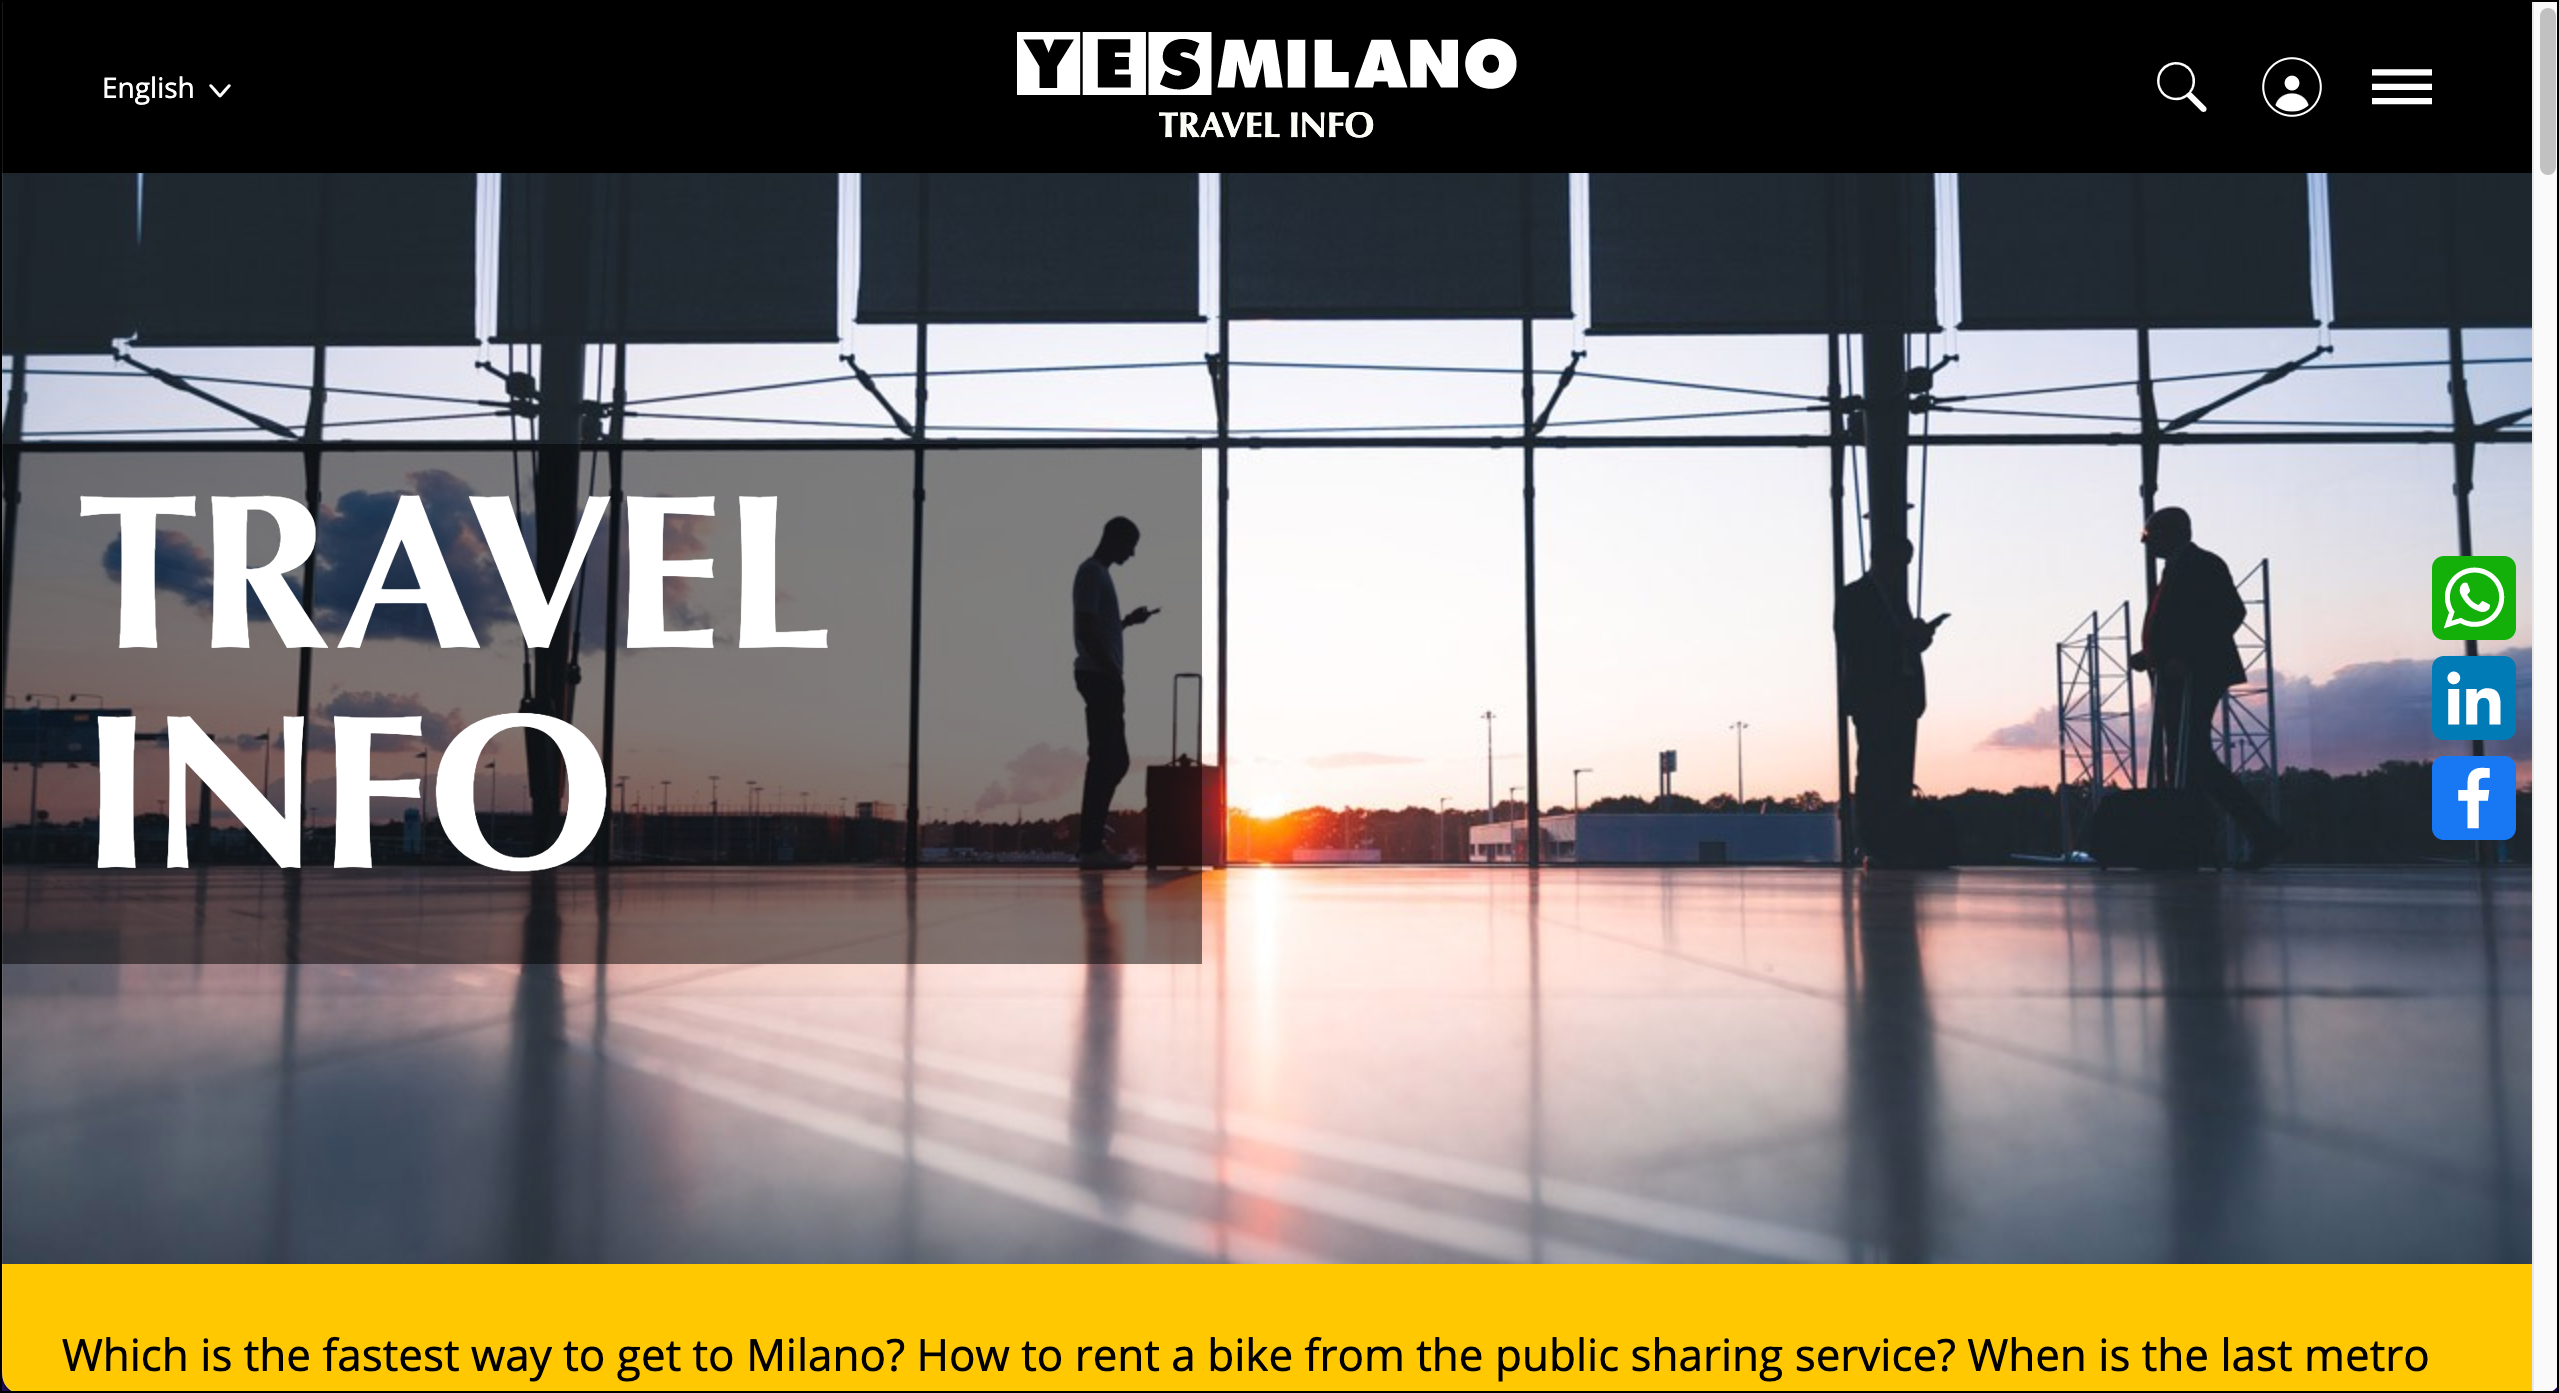
\includegraphics[width=0.5\textwidth]{images/H8-1.png}}%
                \captionsetup{justification=centering}
                \caption{}
                \label{H8-1}
            \end{minipage}
        \end{figure}
        \begin{figure}[!ht]
            \begin{minipage}{\linewidth}
                \centering
                \makebox[\textwidth][c]{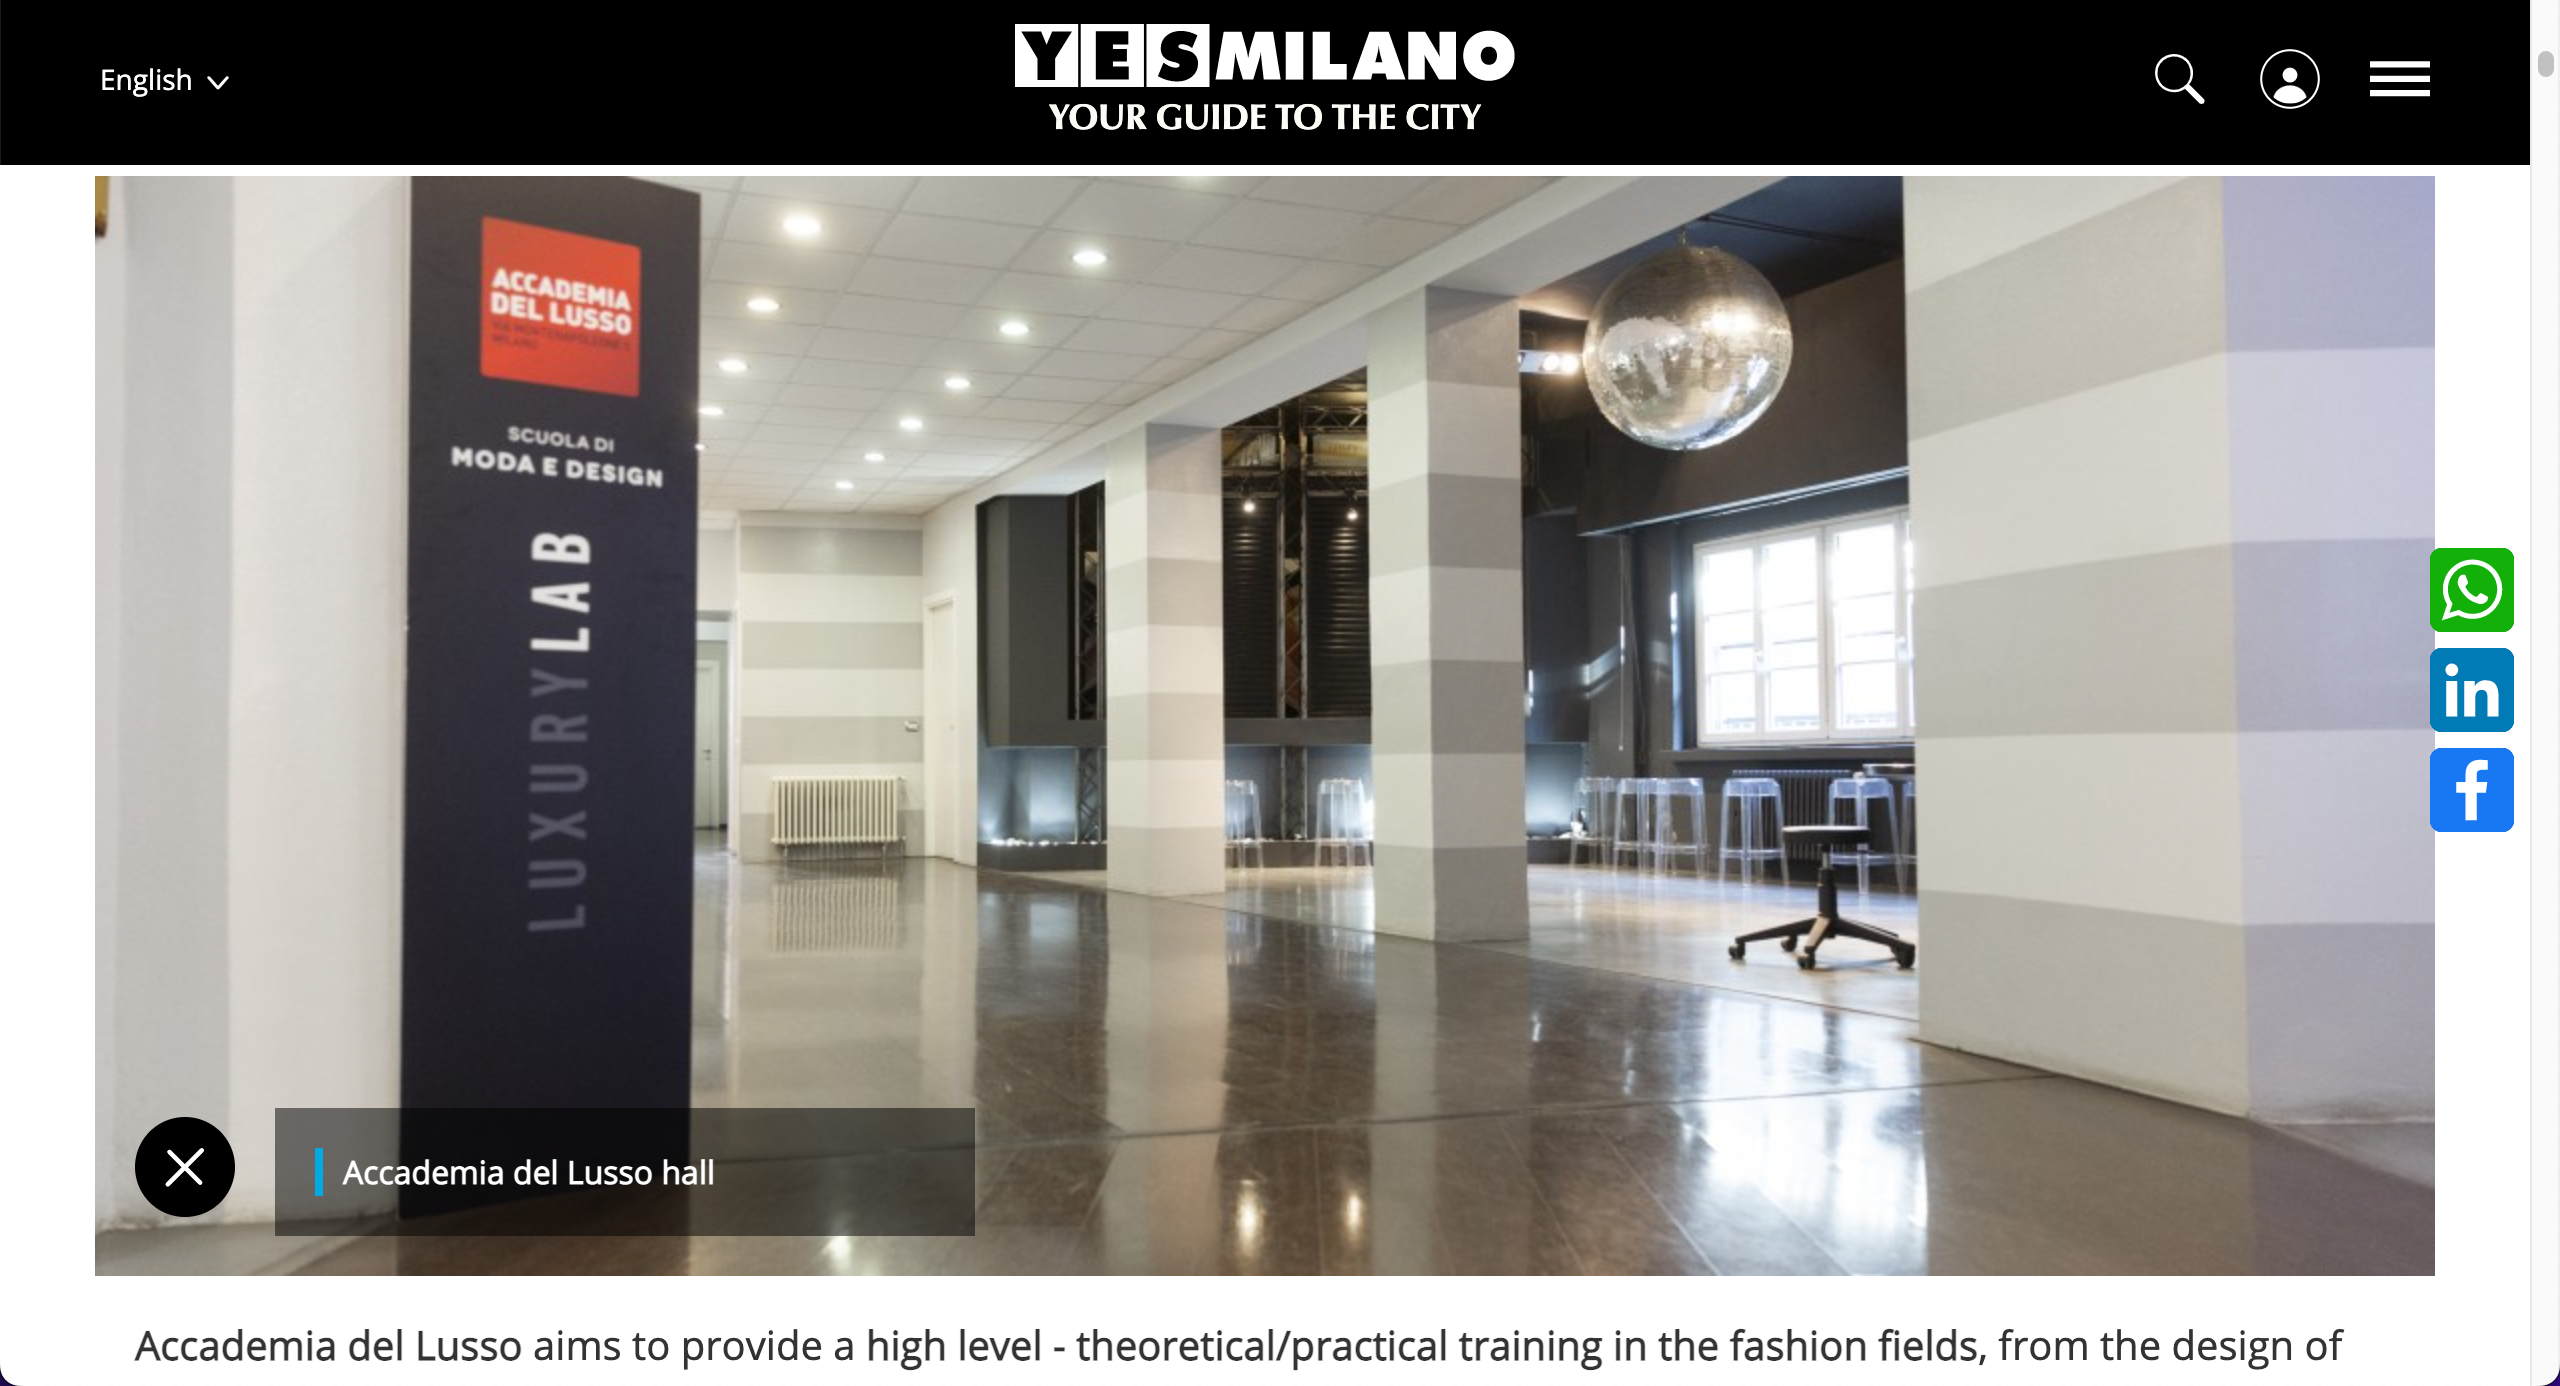
\includegraphics[width=0.5\textwidth]{images/H8-2.png}}%
                \captionsetup{justification=centering}
                \caption{}
                \label{H8-2}
            \end{minipage}
        \end{figure}
    \item \textbf{H9 Help users recognize, diagnose and recover from errors}\\
        In the hotels page, if the geolocalization service fails, the website gives a not helpful error message (See Fig. \ref{H9-1}). Instead in the restaurants page, the same error gives to the user instructions about what to do. (See Fig. \ref{H9-2})\\
        When signing up for the newsletter, if the user first checks the checkbox then no error is shown for leaving the email field blank.\\
        The 404 error message is nicely designed. (See Fig. \ref{H9-3})\\
        The user form registration gives good error feedback. (See Fig. \ref{H9-4})
        \begin{figure}[!ht]
            \begin{minipage}{\linewidth}
                \centering
                \makebox[\textwidth][c]{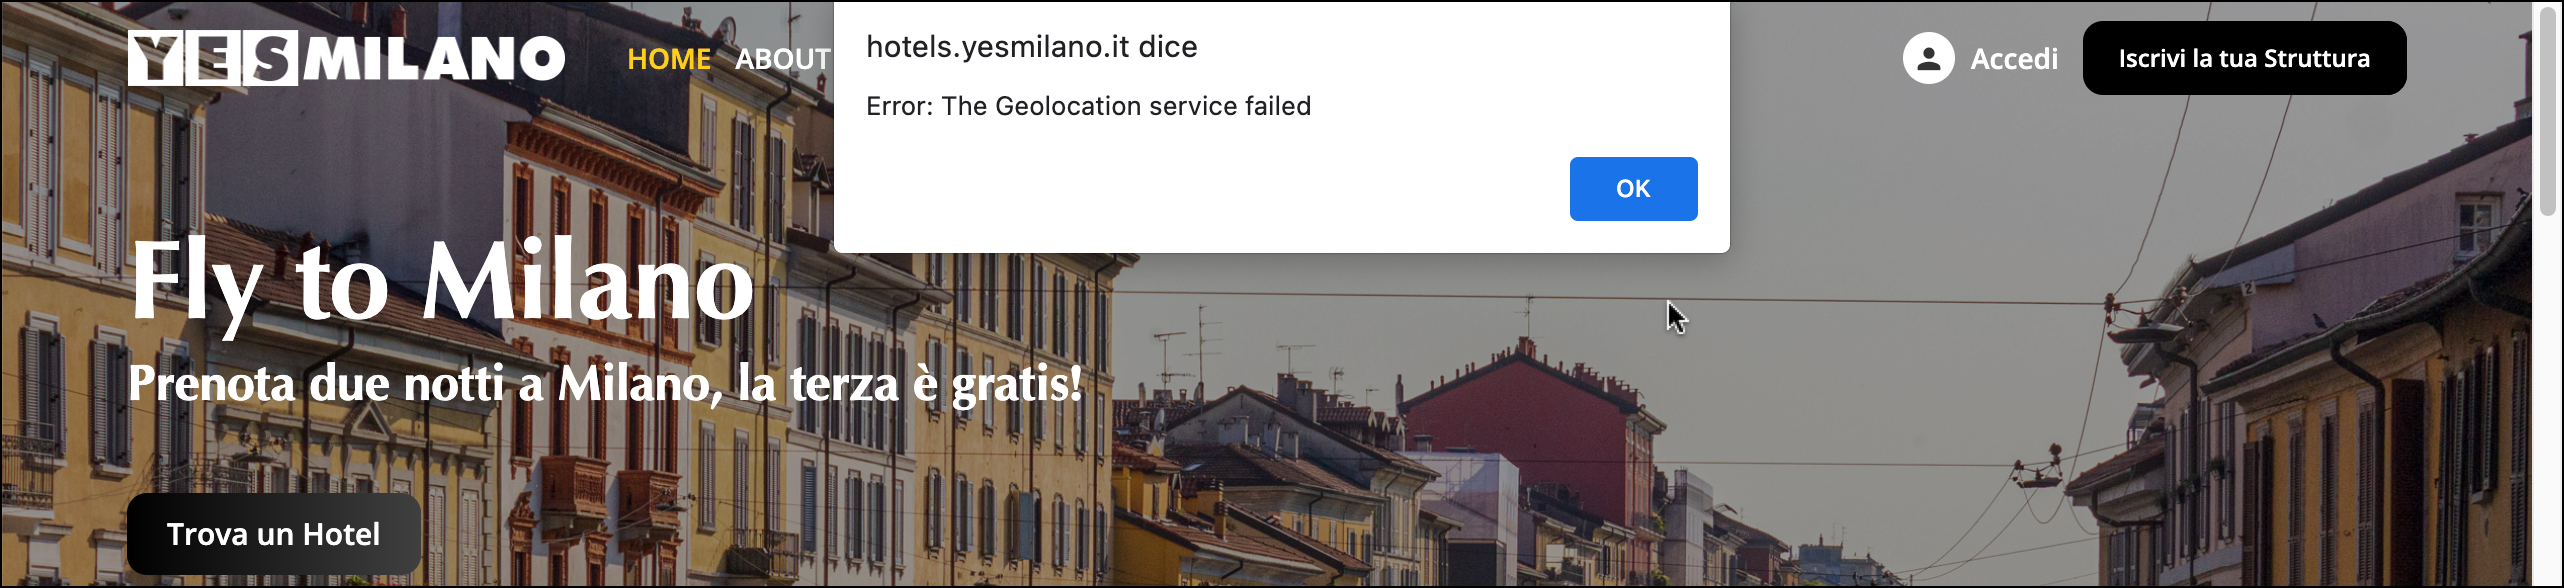
\includegraphics[width=0.5\textwidth]{images/H9-1.png}}%
                \captionsetup{justification=centering}
                \caption{}
                \label{H9-1}
            \end{minipage}
        \end{figure}
        \begin{figure}[!ht]
            \begin{minipage}{\linewidth}
                \centering
                \makebox[\textwidth][c]{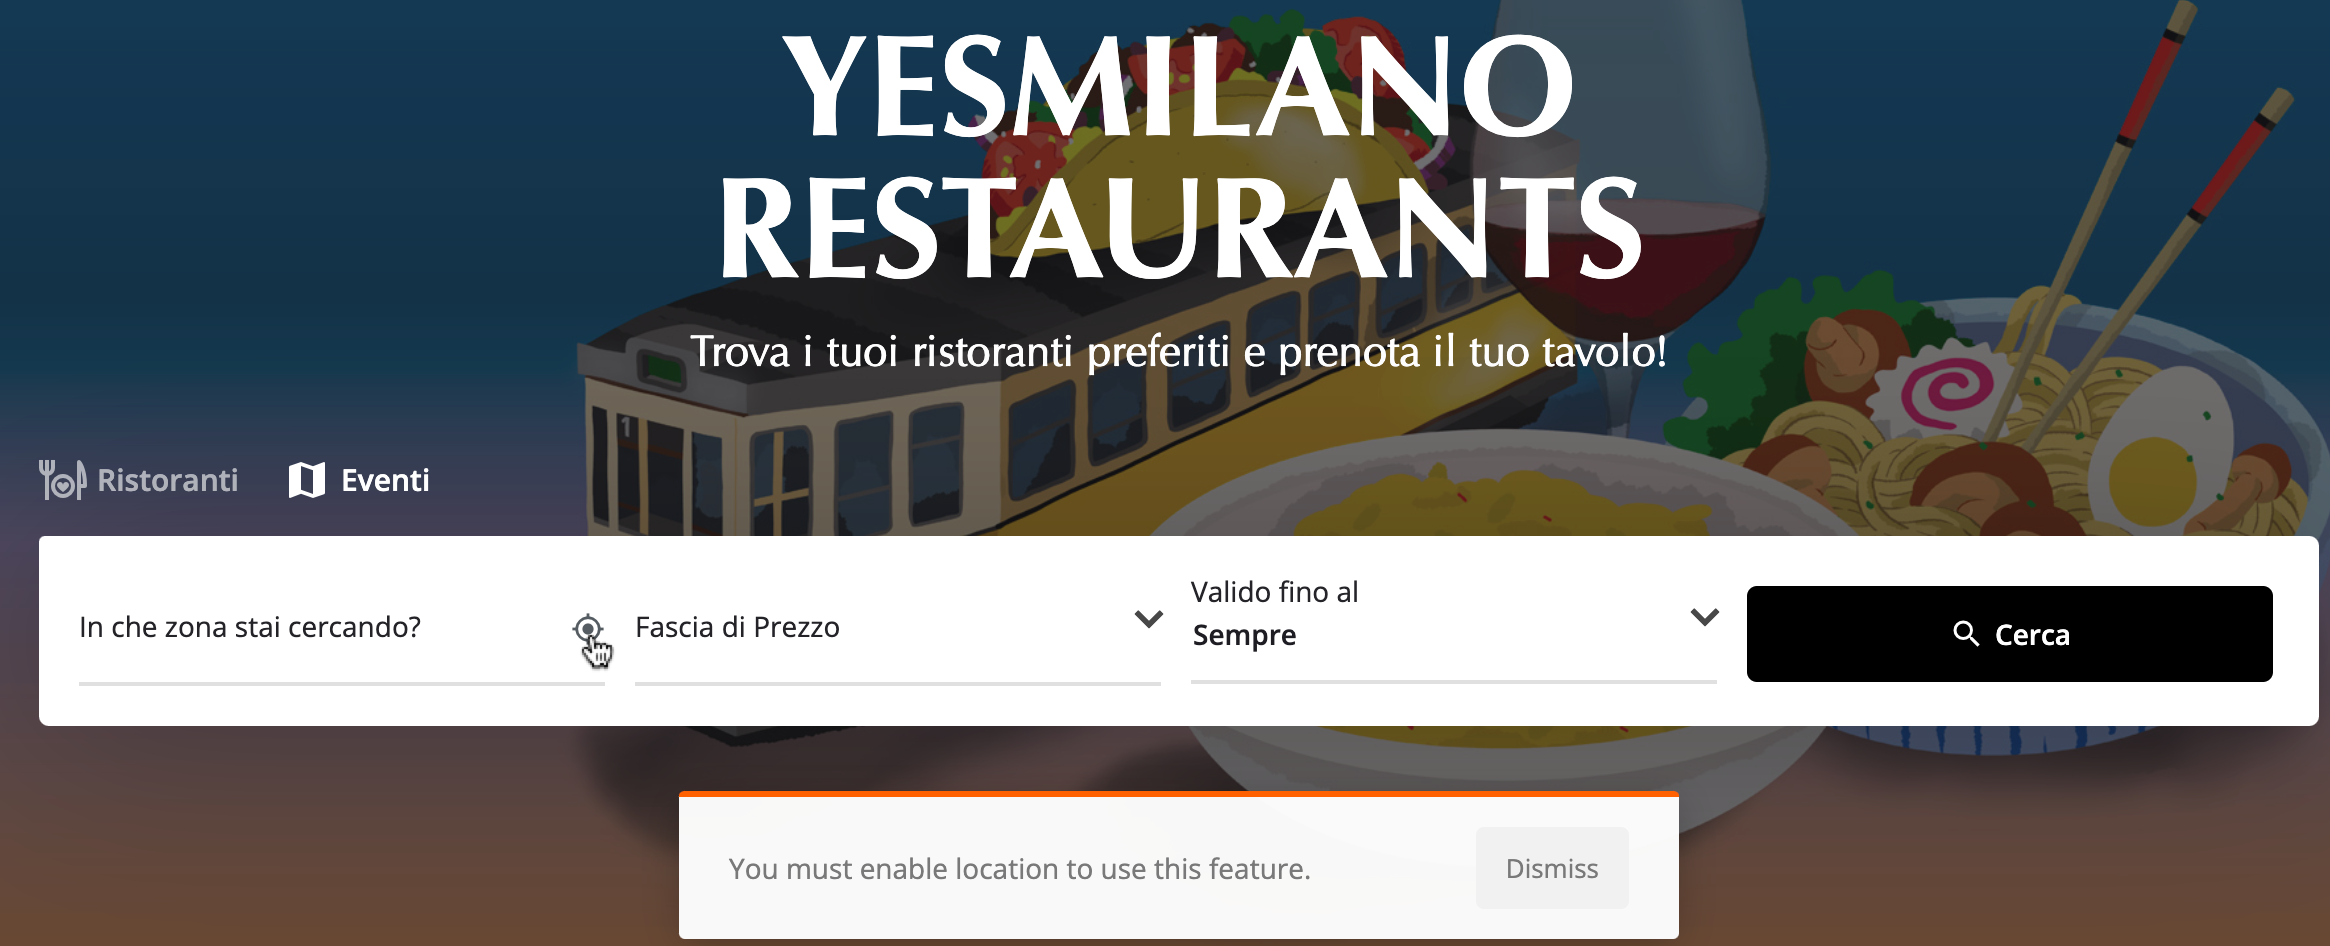
\includegraphics[width=0.5\textwidth]{images/H9-2.png}}%
                \captionsetup{justification=centering}
                \caption{}
                \label{H9-2}
            \end{minipage}
        \end{figure}
        \begin{figure}[!ht]
            \begin{minipage}{\linewidth}
                \centering
                \makebox[\textwidth][c]{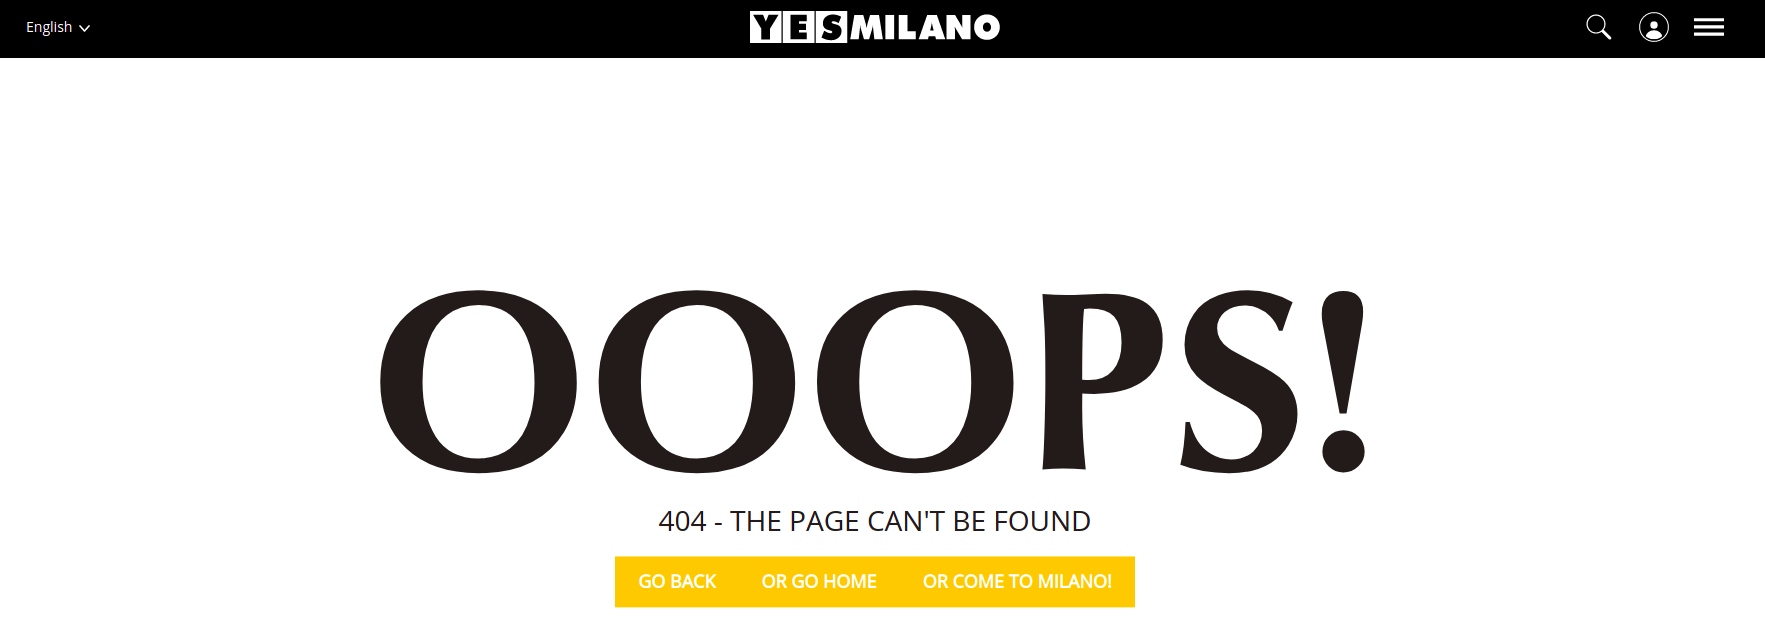
\includegraphics[width=0.5\textwidth]{images/H9-3.png}}%
                \captionsetup{justification=centering}
                \caption{}
                \label{H9-3}
            \end{minipage}
        \end{figure}
        \begin{figure}[!ht]
            \begin{minipage}{\linewidth}
                \centering
                \makebox[\textwidth][c]{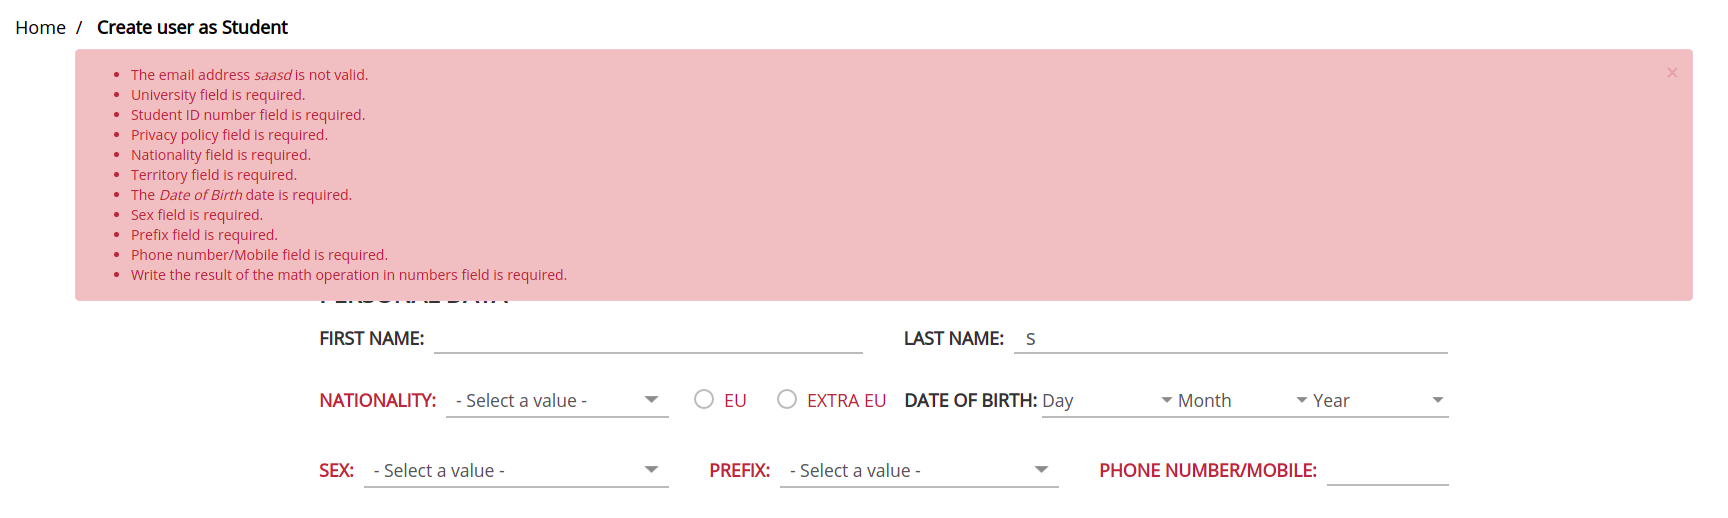
\includegraphics[width=0.5\textwidth]{images/H9-4.png}}%
                \captionsetup{justification=centering}
                \caption{}
                \label{H9-4}
            \end{minipage}
        \end{figure}
    \item \textbf{H10 Help and documentation}\\
        N/A
\end{itemize}

\pagebreak

\subsubsection{Discussion within MiLe's heuristics}
\begin{itemize}
    \item \textbf{MN1 Interaction consistency}\\
        Similar pages have the same type of layout, links and interaction capabilities. Minor differences might be present, however they are not relevant.
    \item \textbf{MN2 Group Navigation}
        In general, it's quite easy to navigate from a group (often a grid or list) to one of its items. The opposite is usually possible through breadcrumbs, although in certain parts of the website (i.e. YesMilano Hotels, Fig. \ref{fig:MN2-1}) there's no way to get back to the group page.
        \begin{figure}[!ht]
            \centering
            \subfloat[][\centering "Explore" page]{{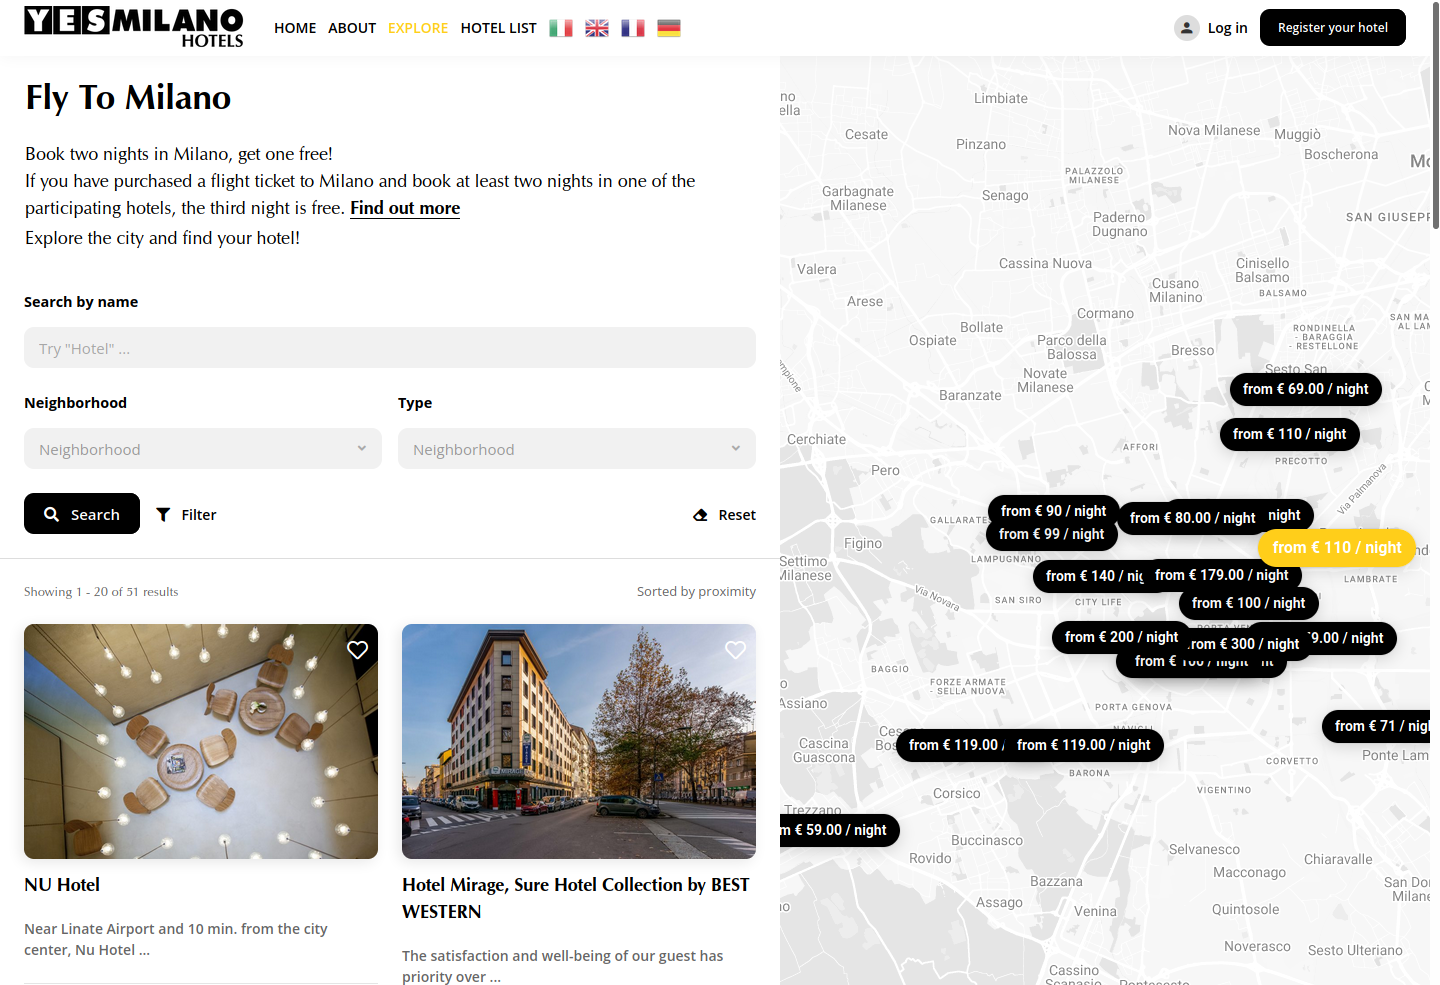
\includegraphics[width=7cm]{images/MN2-1.png} }}%
            \qquad
            \subfloat[][\centering Hotel details page]{{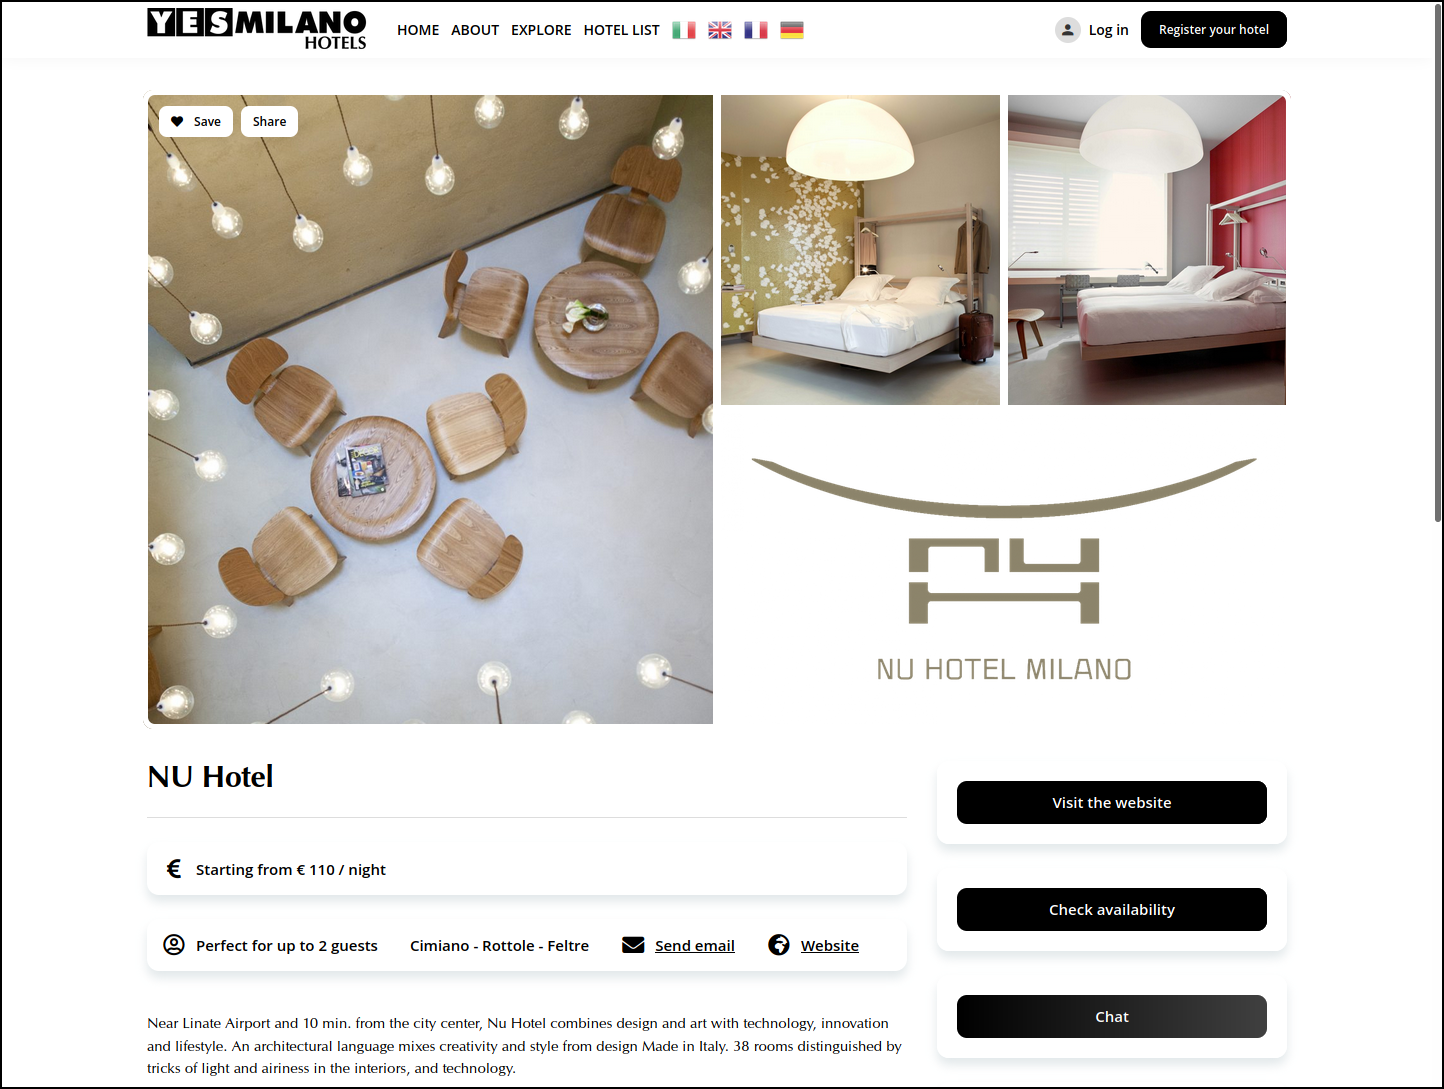
\includegraphics[width=7cm]{images/MN2-2.png} }}%
            \caption{YesMilano Hotes issue with navigation from (b) to (a). To get back the user need to click on the Explore in the header to get back to the hotel list page, which is not obvious.}%
            \label{fig:MN2-1}%
        \end{figure}
    \item \textbf{MN3 Structural Navigation}
        Navigation between parts of a topic could have been better: many pages have a list of same-page links at their top, thus requiring users to scroll back to the top if they want to find a specific section quickly. 

        \begin{figure}[!ht]
            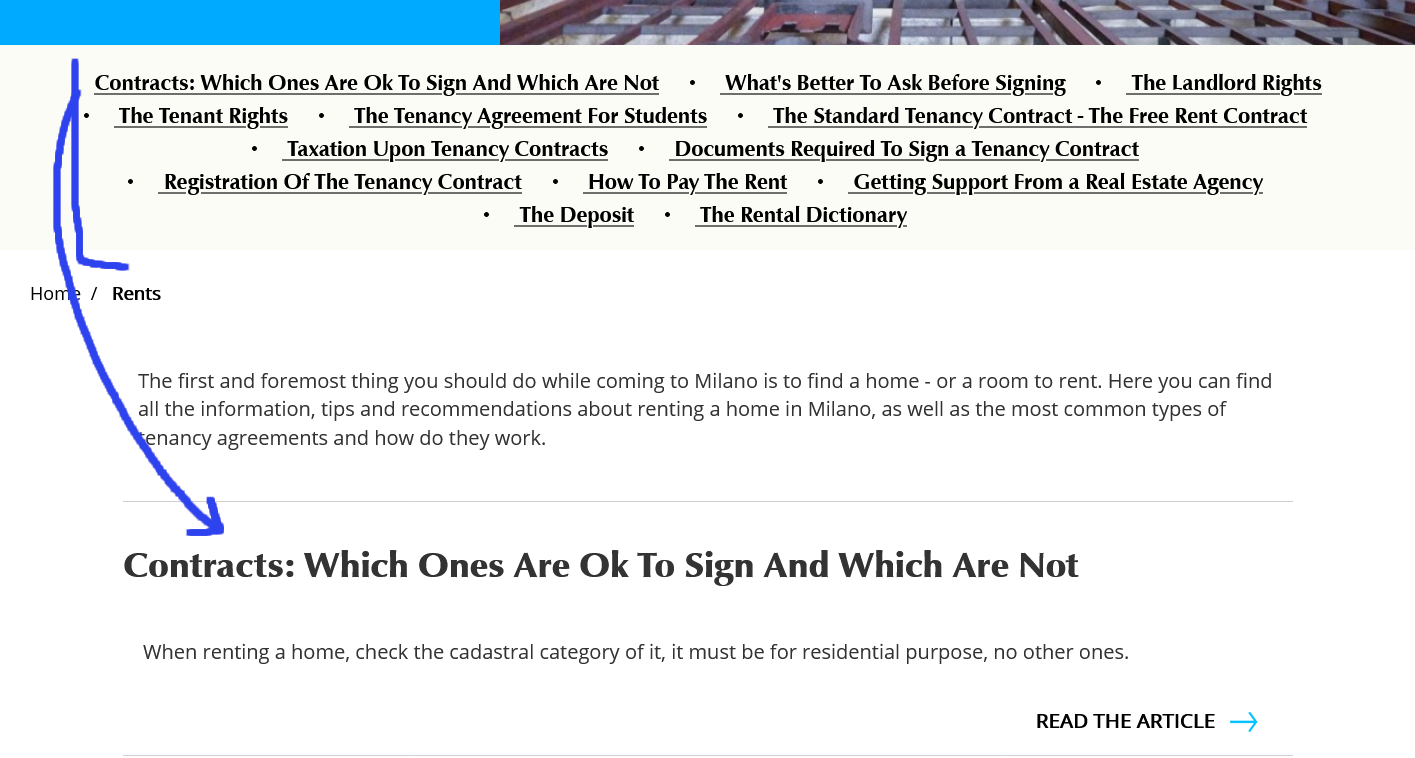
\includegraphics[width=\linewidth]{images/MN3-1.png}
            \caption{From the "Rents" page; the page is quite long and each link points to a section of the page.}
            \label{fig:MN3-1}
        \end{figure} 
    \item \textbf{MN4 Semantic Navigation}
        While it's easy to navigate to related topics thanks to the "You may also like" section of relevant pages, it's not possible to navigate backward to recently visited pages.
    \item \textbf{MN5 Landmarks}
        ???    
    \item \textbf{MC1 Information Overload}
        While most of the website usually presents its contents in a relatively clean way with little bloat, certain pages present their content in a poorly formatted manner. 
        For example, the page that lists universities has a confusing list of links that point to parts of the page, and items like the one in Fig. \ref{fig:MC1-2}, when replicated many times make the page too long.
        While there are sections that present many information in well-organized manner (e.g.: the Coronavirus FAQ page) there are some that present their content with poorly formatted text (e.g.: the "Subway, Trams and Buses" page), as shown in Fig. \ref{fig:MC1-3}.


        \begin{figure}[!ht]
            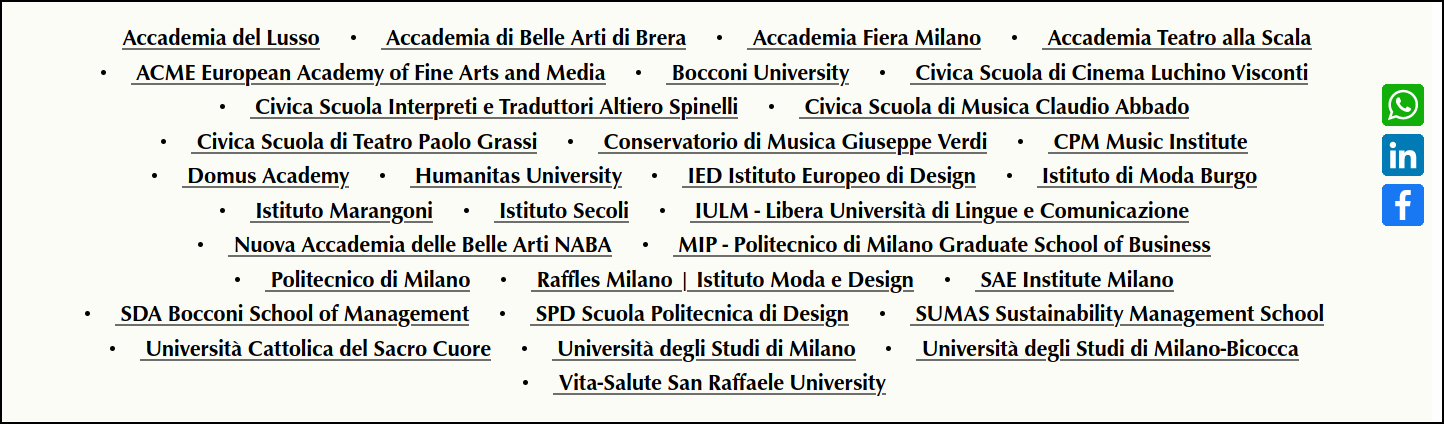
\includegraphics[width=\linewidth]{images/MC1-1.png}
            \caption{The university page list of links.}
            \label{fig:MC1-1}
        \end{figure}
        \begin{figure}[!ht]
            \centering
            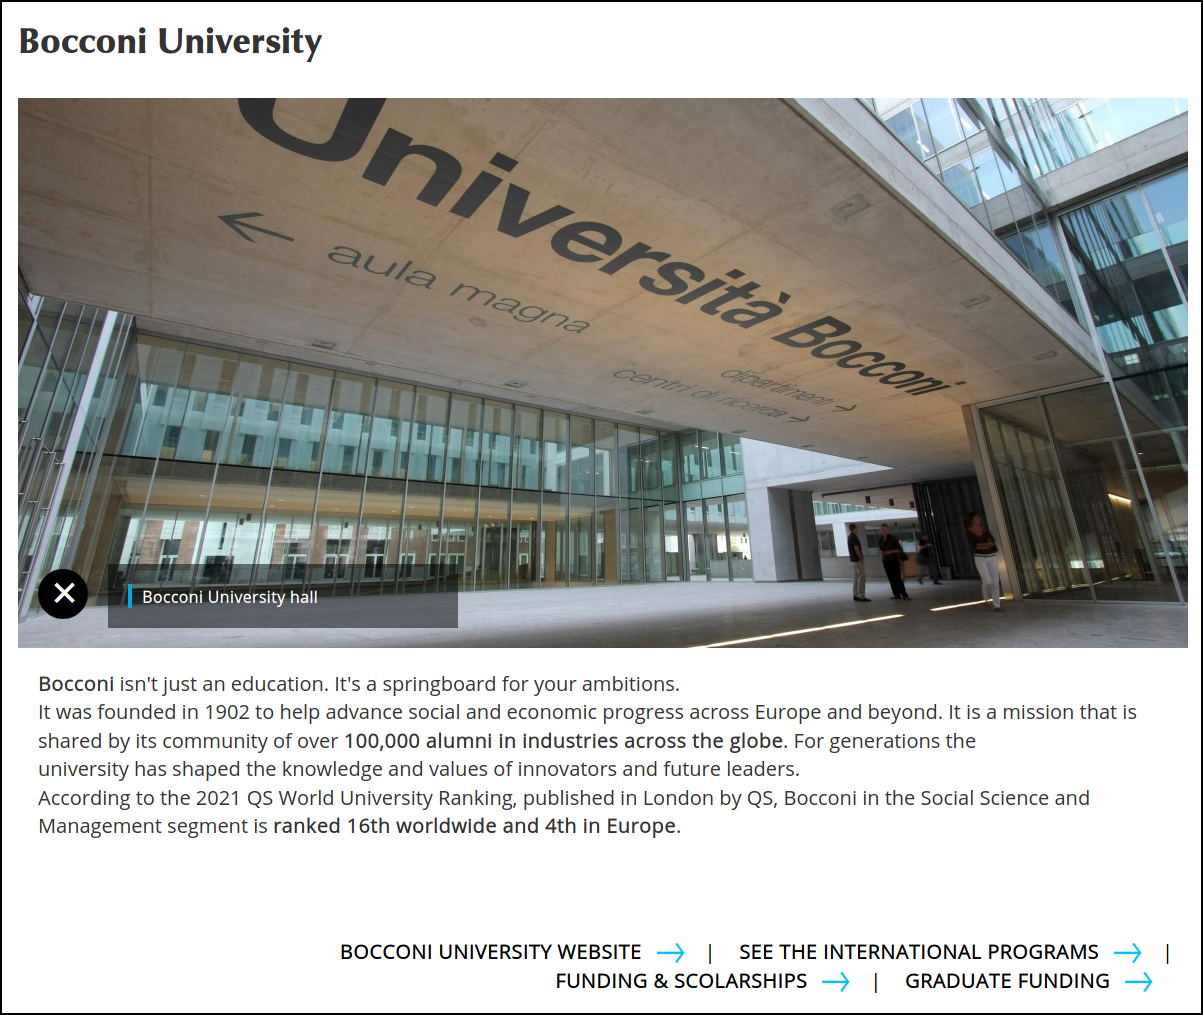
\includegraphics[width=0.7\linewidth]{images/MC1-2.png}
            \caption{An example of an entry of the list of universities.}
            \label{fig:MC1-2}
        \end{figure}
        
        \begin{figure}[!ht]
            \centering
            \subfloat[][\centering Coronavirus FAQ page]{{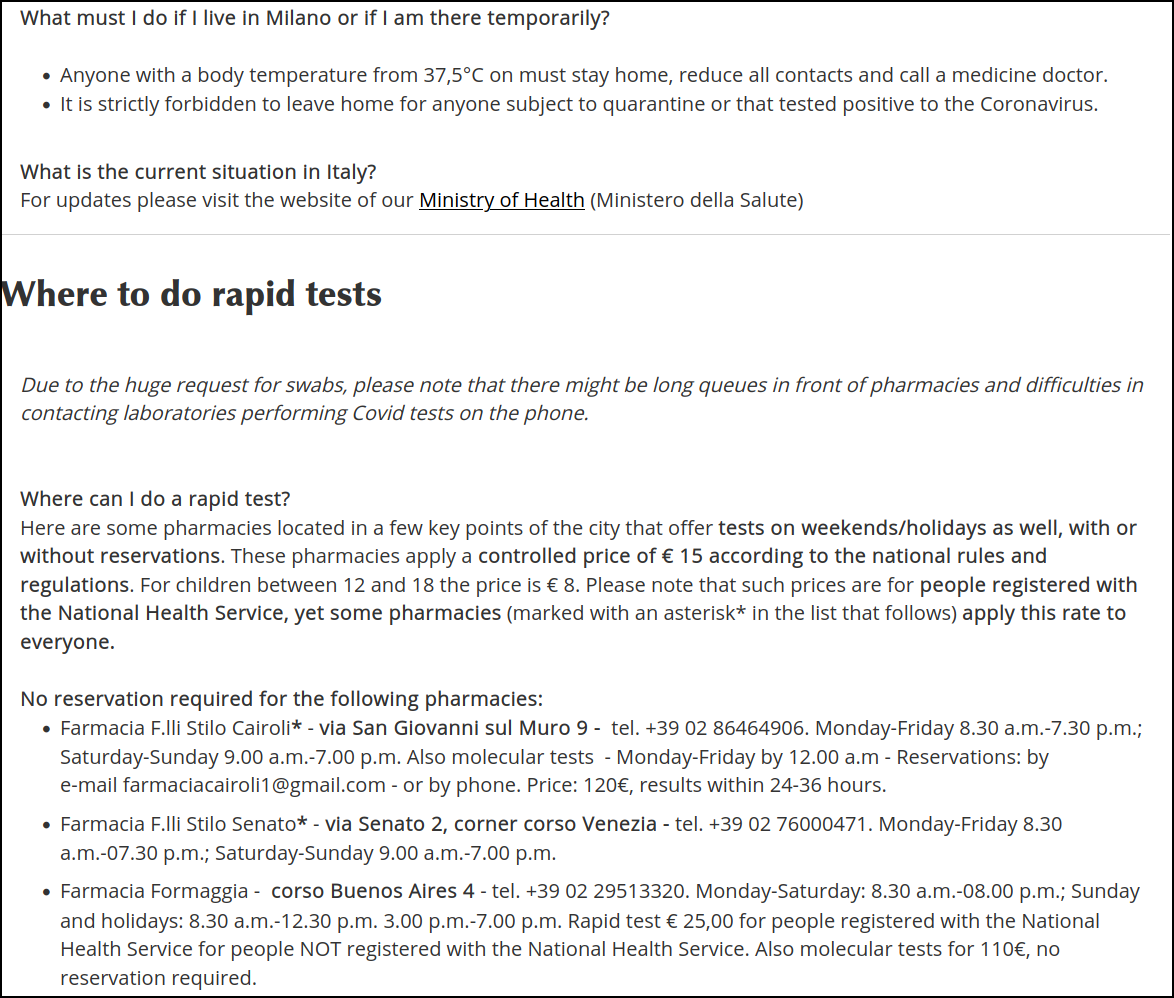
\includegraphics[width=7cm]{images/MC1-4.png} }}%
            \qquad
            \subfloat[][\centering Subway, Trams and Buses]{{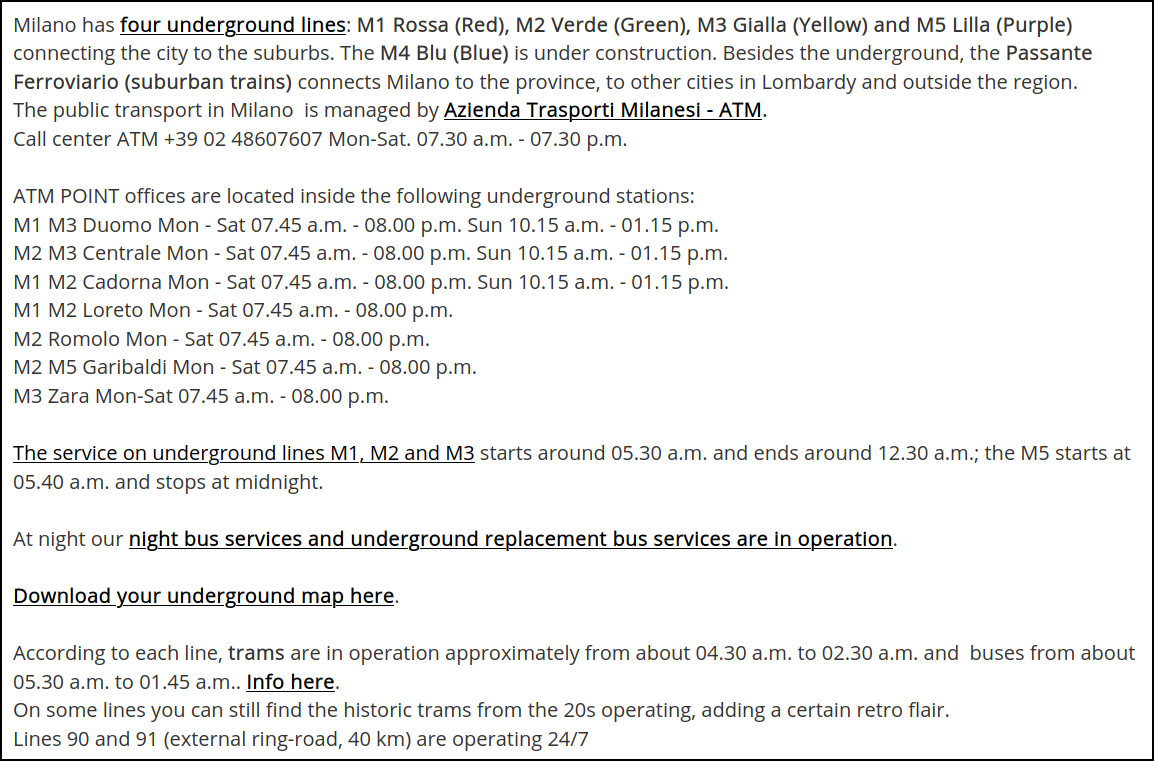
\includegraphics[width=7cm]{images/MC1-3.png} }}%
            \caption{The page on the left make adequate use of heading, lists and different text formatting to highlight different sections of the text, while the page on the right does not.}%
            \label{fig:MC1-3}%
        \end{figure}
    \item \textbf{MP1 Text lay out}\\
        We haven't found any critical aspect, the text is always readable and of the appropriate size.\\
    \item \textbf{MP2 Interaction placeholders-semiotics}\\
        We detected a number of minor problems in this heuristic: some icons are mismatched with regards to their meaning, and there are labels that are unclear in their functionalities (Fig. \ref{MP2-1} and \ref{MP2-2})
        \begin{figure}[!ht]
            \begin{minipage}{\linewidth}
                \centering
                \makebox[\textwidth][c]{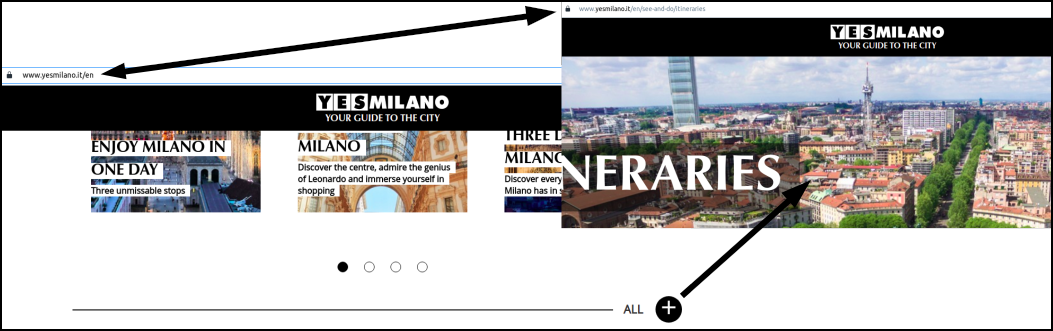
\includegraphics[width=1.2\textwidth]{images/MP2-1.png}}%
                \captionsetup{justification=centering}
                \caption{Conventionally, the "+" should expand the page,\\
                but in the home page it leads to a new page}
                \label{MP2-1}
            \end{minipage}
        \end{figure}
        \begin{figure}[!ht]
            \begin{minipage}{\linewidth}
                \centering
                \makebox[\textwidth][c]{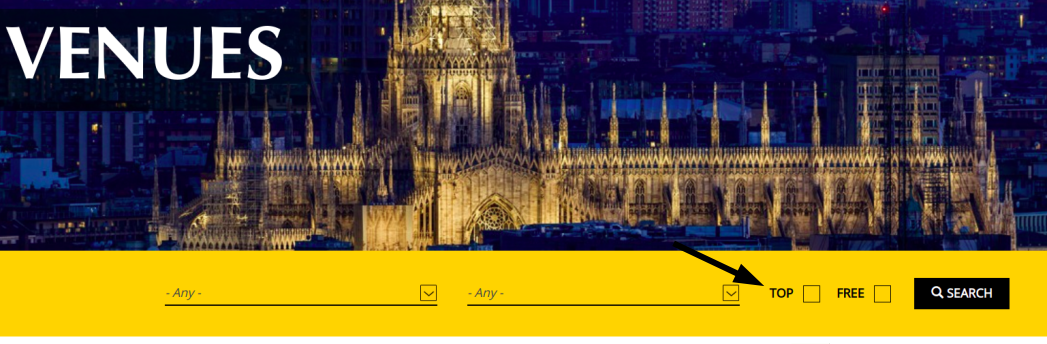
\includegraphics[width=1\textwidth]{images/MP2-2.png}}%
                \captionsetup{justification=centering}
                \caption{In the venues form page, it's unclear what does "TOP" mean in this context.\\If it's based on users reviews, there is no rating system explained}
                \label{MP2-2}
            \end{minipage}
        \end{figure}
    \item \textbf{MP3 Interaction placeholders-consistency}\\
        Some minor problems were found in this heuristic:
        a number of icons are used with multiple meanings (for example the "+" sometimes expands a paragraph section, other times it leads to a new page like in Fig \ref{MP2-1}), and many interactive labels providing the same functionalities are named differently across the same page (Fig. \ref{MP3-1} and Fig. \ref{MP3-2}).
        \begin{figure}[!ht]
            \begin{minipage}{\linewidth}
                \centering
                \makebox[\textwidth][c]{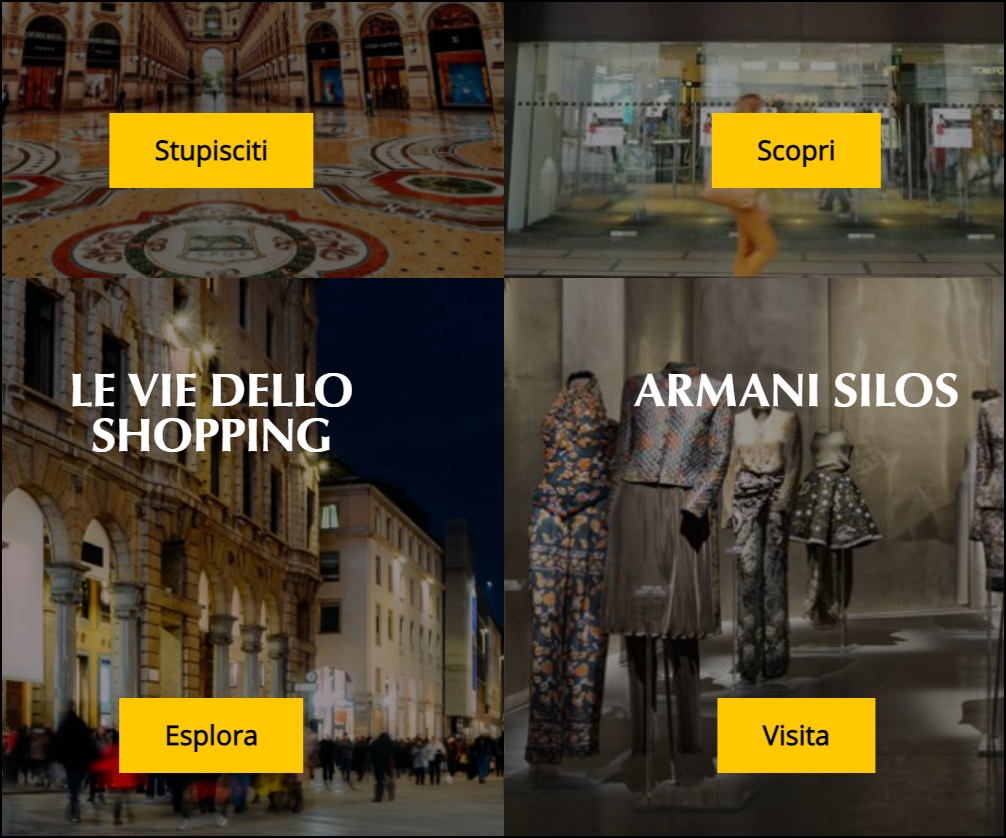
\includegraphics[width=0.5\textwidth]{images/MP3-1.png}}%
                \captionsetup{justification=centering}
                \caption{In the Fashion \& Shopping page, interactive labels are equivalent in terms of functionalities are named differently, sometimes even in confusing ways ("Stupisciti" which translates to "Amaze yourself" it's not really suggestive of its functionality)}
                \label{MP3-1}
            \end{minipage}
        \end{figure}
        \begin{figure}[!ht]
            \begin{minipage}{\linewidth}
                \centering
                \makebox[\textwidth][c]{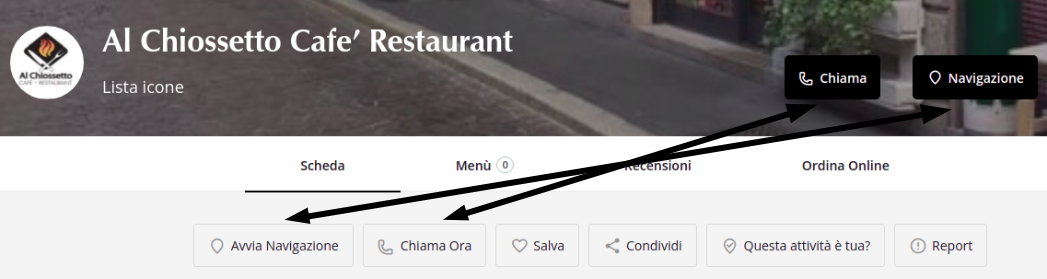
\includegraphics[width=1\textwidth]{images/MP3-2.png}}%
                \captionsetup{justification=centering}
                \caption{In any dedicated restaurant page, interactive elements\\for contacting and locating the place are labeled differently}
                \label{MP3-2}
            \end{minipage}
        \end{figure}
        \pagebreak
    \item \textbf{MP4 Spatial allocation}\\
        The overall allocation of elements in each page is good, but a critical aspect lowered the score: the venues form page through which the user can retrieve venues through various filters has an anchor in the footer only ("All the venues", Fig. \ref{MP4-1}). Given the importance of such page, the lack of a link in the top menu is a major problem that even affects the navigation.\\
        Other problems are the positioning of the partners logos and links which precede the more important footer links (Fig. \ref{MP4-1})), and the placing of the anchors leading to sections of the same page (Fig. \ref{MP4-2}): as their role is simplifying navigation, allocating them at the top of the page only is not very appropriate as the user is forced to scroll all the way back to the top just to change section.
        \begin{figure}[!ht]
            \begin{minipage}{\linewidth}
                \centering
                \makebox[\textwidth][c]{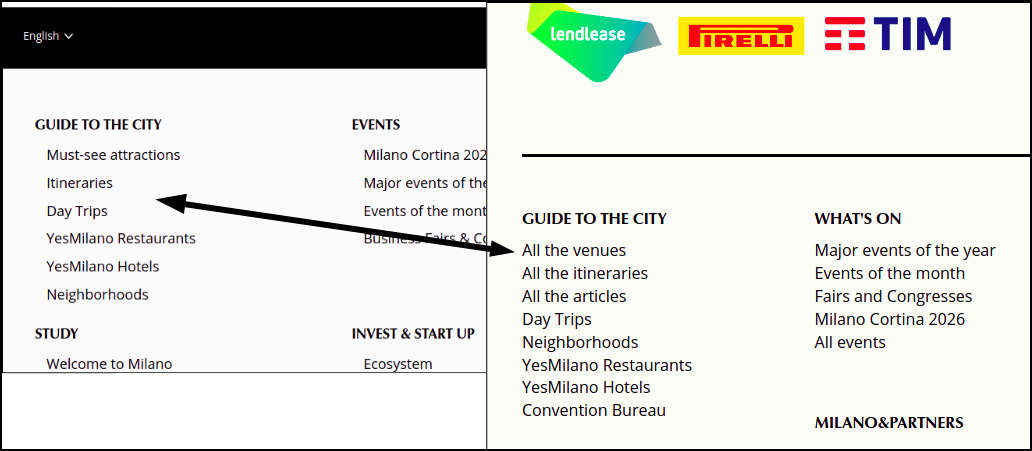
\includegraphics[width=1\textwidth]{images/MP4-1.png}}%
                \captionsetup{justification=centering}
                \caption{"All the venues" link present only in the footer\\Partners' logos precede footer links}
                \label{MP4-1}
            \end{minipage}
        \end{figure}
        \begin{figure}[!ht]
            \begin{minipage}{\linewidth}
                \centering
                \makebox[\textwidth][c]{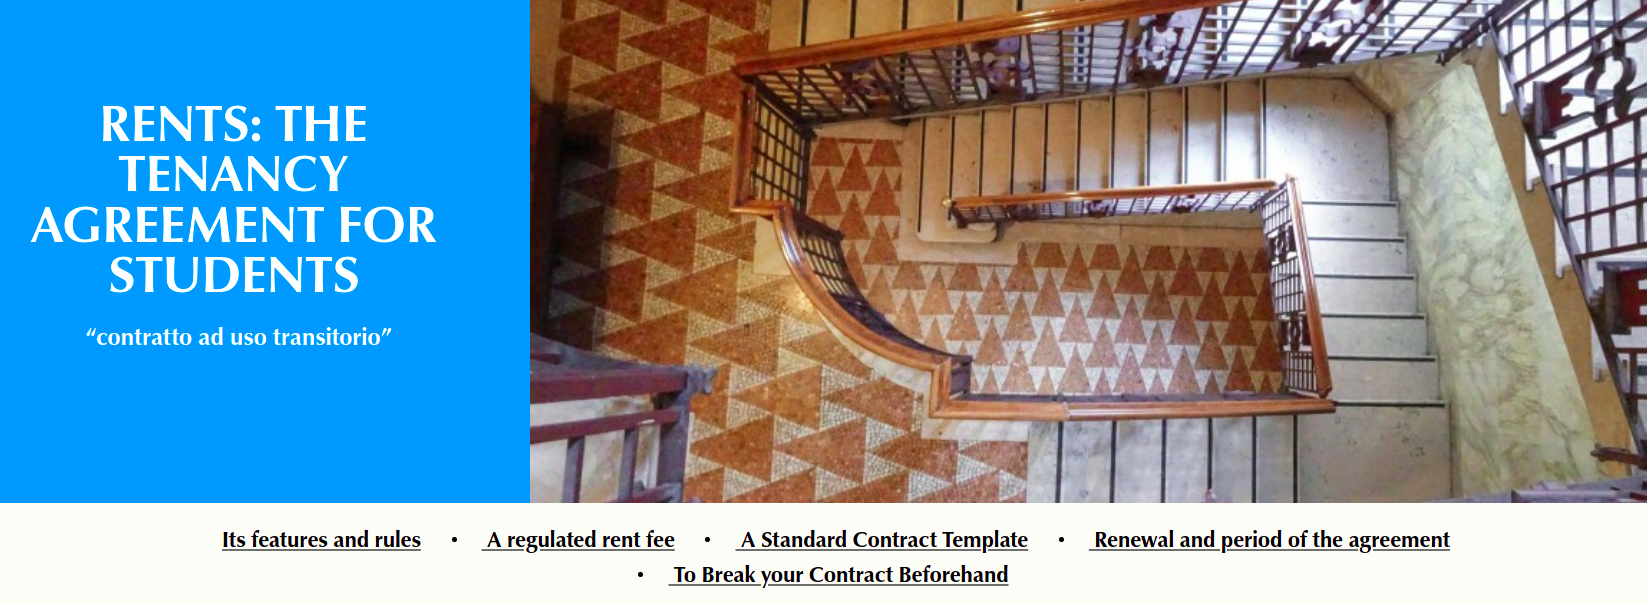
\includegraphics[width=1\textwidth]{images/MP4-2.png}}%
                \captionsetup{justification=centering}
                \caption{This anchors placement hardens the navigation aspect too\\A solution would be making them sticky (always on top of page) or putting them in a side bar}
                \label{MP4-2}
            \end{minipage}
        \end{figure}
    \item \textbf{MP5 Consistency of Page Structure}\\
        We didn't detect major problems in this aspect, pages of the same type have the same layout.\\
        For example, all venues' pages have a brief initial paragraph describing the attraction, a middle section with various useful information like contancts, schedule and pricing, and finally a final part of the page is dedicated to suggestions. 
\end{itemize}